\documentclass{article}

\usepackage{graphicx}
\usepackage{subcaption}
\usepackage{tikz}
\usepackage[utf8]{inputenc}
\usepackage[T1]{fontenc}
\usepackage{lmodern}
\usepackage{amsmath}
\usepackage{amsthm}
\usepackage{amsfonts}
\usepackage{amssymb}
\usepackage{enumitem}
\usepackage{commath}
\usepackage{mathtools}
\usepackage{adjustbox}
\usepackage{setspace}
\usepackage{bigints}
\usepackage{hyperref}
\usepackage{ulem}
\usepackage{esdiff}
\usepackage{pgfplots}
\usepackage{caption}
\usetikzlibrary{shapes.symbols, positioning}
\usepackage{tikz-cd}
\usetikzlibrary{positioning}



\newtheorem{definicija}{Definicija}
\newtheorem{trditev}{Trditev}
\newtheorem{lema}{Lema}
\newtheorem{posledica}{Posledica}
\newtheorem{opomba}{Opomba}
\newtheorem{primer}{Primer}
\newtheorem{izrek}{Izrek}


\newcommand{\C}{\mathbb{C}}
\newcommand{\Z}{\mathbb{Z}}
\newcommand{\N}{\mathbb{N}}
\newcommand{\M}{\mathcal{M}}
\newcommand{\R}{\mathbb{R}}
\newcommand{\Ho}{\mathcal{O}}
\newcommand{\dd}{\mathrm{d}}

\title{Dinamika realnih funkcij}
\author{Uroš Kosmač}

\begin{document}

% Create a new 1st level heading
\section{Uvod}
Kaj so dinamični sistemi? Najbolj enostavno jih lahko opišemo kot:\\[1mm]
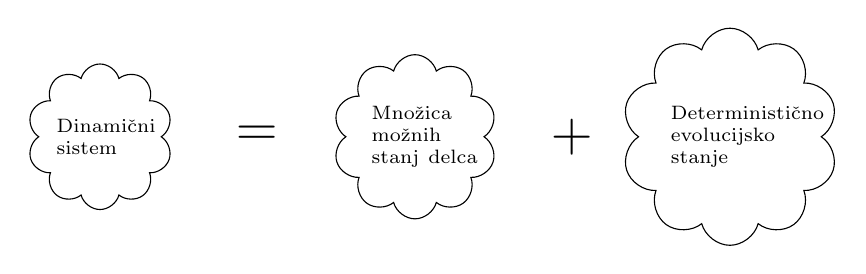
\begin{tikzpicture}
    \node[text width=1.1cm,inner sep=0pt]
    [execute at begin node=\setlength{\baselineskip}{8pt},
        cloud,
        draw] (c) at (0,0)
    {\scriptsize{Dinamični\\sistem}};
    \node at (2,0) {\huge $=$};
    \node[text width=1.1cm,inner sep=2pt]
    [execute at begin node=\setlength{\baselineskip}{8pt},
        cloud,
        draw] (c) at (4,0)
    {\scriptsize{Množica možnih\\ \text{stanj delca}}};
    \node at (6,0) {\huge $+$};
    \node[text width=1.5cm,inner sep=2pt]
    [execute at begin node=\setlength{\baselineskip}{8pt},
        cloud,
        draw] (c) at (8,0)
    {\scriptsize{Deterministično evolucijsko\\stanje}};
\end{tikzpicture}
~\\[1mm]
Drugače povedano, obravnavamo delec v množici možnih stanj, pravilo, pa nam pove, kaj se z njim zgodi v naslednjem trenutku.\\ 
Deterministično, v našem kontekstu pomeni, da je naslednji korak odvisen le od trenutnega stanja delca.\\ 
V grobem jih glede na tip koraka, ločimo na \textbf{diskretne} in \textbf{zvezne} sisteme. V splošnem jih lahko obravnavamo na npr. metričnih ali topoloških prostorih, mi pa se bomo omejili na $\R^n$ in $\C$. Obravnavali bomo
\begin{enumerate}
\item[i)] Diferenčne oz.rekurzivna enačbe $x_{n+1} = F(x_n)$, 
za $F: S\rightarrow S$ in pri različnih začetnih pogojih $x_0 \in S$, kjer je $S$ množica stanja v $\R^n$ ali $\C$. Temu rečemo diskretna dinamika funkcije oz. preslikave $F$
\item[ii)] Nelinearni sistemi navadnih diferencilnih enačb, $F: S\subseteq \R^n \rightarrow S \subseteq \R^n$, $\dot{x} = F(x)$, $x\in S$. To bo model za zvezne dinamične sisteme v $\R^n$.
\end{enumerate}

\begin{opomba}
V obeh primer govorimo o \textbf{autonomnih sistemih} tj. pravilo ni odvisno od časa. Pokažimo, da lahko poljuben sistem prevedemo na avtonomen sistem, zato je dovolj obravnavati le te.
\begin{align*}
\dot{x} = F(x,t) \iff  &\dot{x} = F(x, t) \iff \dot{\tilde{x}} = \tilde{F}(\tilde{x}) \text{ za } \tilde{x} = (x, t) \text{ in } \tilde{F} = (F, 1) \\ 
&\dot{t} = 1
\end{align*}

\begin{align*}
x_{n+1} = F(x_n,n) \iff  &x_{n+1} = F(x_n, y_n) \iff \tilde{x}_{n+1} = \tilde{F}(x_n) \text{ za } \tilde{x} = (x, y) \\ 
                         &y_{n+1} = y_n + 1
\end{align*}

tj. če nimamo dimenzijskih omejitev, so avtonomni sistemi najsplošnejši možni, saj lahko čas premaknemo v množico stanj tj. $\tilde{S} = S \times \R$ oz. $\tilde{S} = S \times \Z$.
\end{opomba}

\begin{primer}
Zgodil se je umor in imamo naslednje podatke:
\begin{itemize}
    \item Temperatur $T$ trupla ob prihodu: $T(0) = 9^\circ C$
    \item Temperatura $T$ po $1$h: $T(1) = 7^\circ C$
    \item Temperatura jezera $T_j$: $T_j = 5^\circ C$ 
\end{itemize}
Kdaj se je zgodil umor? \\
Fizikalni zakon: telesna temperatura pada sorazmerno z razliko do temperature jezera. \\
Diskretni model:
$$
T_{n+1} = T_n - k(T_n - T_j),
$$
kjer sta:
\begin{itemize}
\item $k>0$ konstanta odvisna le od lasnosti trupla
\item $T_n - T_j$ temperaturna razlika
\end{itemize}
Vstavimo meritve: čas ob prihodu
\begin{align*}
7C &= 9C - k(9C - 5C) \\ 
&\Longrightarrow k = \frac{1}{2}.
\end{align*}
Sistem, ki opisuje telesno temperaturo, je podano z 
$$
T_{n+1} = T_n - \frac{1}{2}(T_n - T_j) = \frac{1}{2}T_n + \frac{1}{2} T_j.
$$
\noindent
V tem primeru lahko poiščemo ekplicitno rešitev:\\ 
Homogeni del:
$$
T_{n+1} = \frac{1}{2} T_n \Longrightarrow T_n = C\Big(\frac{1}{2}\Big)^n.
$$
Partikularna rešitev:
$$
T_n^p = T_j = 5C
$$
Splošna rešitev:
\begin{align*}
T_n &= C\Big(\frac{1}{2}\Big)^n + T_j \\ 
T_0 &= C + T_j \Longrightarrow C = T_0 - T_j\\ 
T_n &= (T_0 - T_j)\cdot\Big(\frac{1}{2}\Big)^n + T_j
\end{align*}
Odgovor:\\ 
vemo, da je $T_0 = 37C$ torej imamo
\begin{align*}
T_n &= (37 - 5) \Big(\frac{1}{2}\Big)^n  + 5 = 9 \\ 
&\Longrightarrow n = 3.
\end{align*}
Umor se je zgodil $3h$ pred prihodom.\\ 
Zvezni model:
model je dan z
$$
\dot{T} = - k(T - T_j).
$$
Rešimo z metodo ločljivih spremenljiv
$$
T = D e^{-kt} + T_j
$$
Začetni pogoj: $T(0) = T_0$ $\Longrightarrow$ $D = T_0 - T_j$ in je rešitev
$$
T(t) = (T_0 - T_j)e^{-kt} + T_j
$$
Čas prihoda: $T(n) = 9C$, \\ 
Čas po eni uri: $T(n+1) = 7C$.\\ 
Rešimo sistem enačb in dobimo $n = 3$. Dobimo enak sklep kot prej, dinamični sistem, ki opisuje temperaturo, pa je
$$
\dot{T} = \ln\Big(\frac{1}{2}\Big)(T - T_j) = -\ln{2}(T-T_j)
$$
\begin{tikzpicture}
    \begin{axis}[
        axis x line=middle, 
        axis y line=middle,
        xlabel={$t$}, ylabel={$T$},
        xmin=0, xmax=5, ymin=0, ymax=3,
        samples=100,
        domain=0:5,
        legend pos=south east
    ]
        % Asymptote T_j
        \addplot[dashed] coordinates {(0,2) (5,2)} node[pos=1,right] {$T_j$};
        
        % Logarithmic-type curves converging to T_j from below
        \addplot[thick,blue] {2 - 0.8*exp(-x)};
        \addplot[thick,red] {2 - 1.2*exp(-x)};
        \addplot[thick,green] {2 - 0.5*exp(-x)};
        
        % Logarithmic-type curves converging to T_j from above
        \addplot[thick,purple] {2 + 0.6*exp(-x)};
        \addplot[thick,orange] {2 + 0.9*exp(-x)};
        
        % Marking initial values t_0
        \node[blue] at (15, 140) {$t_0$};
        \node[red] at (15, 110) {$t_0$};
        \node[green] at (15, 170) {$t_0$};
        \node[purple] at (15, 240) {$t_0$};
        \node[orange] at (15, 270) {$t_0$};
        
    \end{axis}
\end{tikzpicture}


\vspace{1cm}
V tem primeru, je $T \equiv 5C$ neka fiksna točka oz. ravnovesje, "pritegne" ostale rešitve. Tekom predmeta bomo spoznali bolj zapletene primere.
\end{primer}

\maketitle
\section{Osnovni pojmi}
Za začetek se bomo omejili na funkcije $f: I\subseteq \R \rightarrow I$, kjer je $I$ interval. Obravnavali bomo zaporedje $x_{n+1} = f(x_n)$ pri različnih pogojih $x_0 \in I$. Za začetek uvedemo oznako:
$$
f^n = \underbrace{f\circ f \dots \circ f}_{n \text{ kompozitumov} }
$$
\begin{definicija}
\textbf{Orbita točke $x_0$} pri funkciji $f$ je podana s členi zaporedja:
$$
O_f(x_0) = \{x_0, x_1, \dots\} = \{f^n(x_0)\,|\, n\in \N_0\}.
$$
Orbita predstavlja dinamični razvoj točke $x_0$ pri komponiranju z $f$. 
Množici vseh orbit za $x_0 \in I$ pa rečemo \textbf{dinamika funkcije $f$}.
\end{definicija}

\begin{primer}
$x_{n+1} = x_n^2 + 1 \text{ oz. } f(x) = x^2 + 1$
\begin{align*}
O_f(1) &= \{1, 2, 5, 26, \dots\} \\ 
O_f(0) &= \{0, 1, 2, 5, 26, \dots\}\\
O_f(-2) &= \{-2, 5, 26, \dots \}
\end{align*}
orbite lahko pri funkcijah ene spremenljivke vizualiziramo z \textbf{pajčevinastim diagramom}.

\begin{figure}[h]
\begin{centering}
    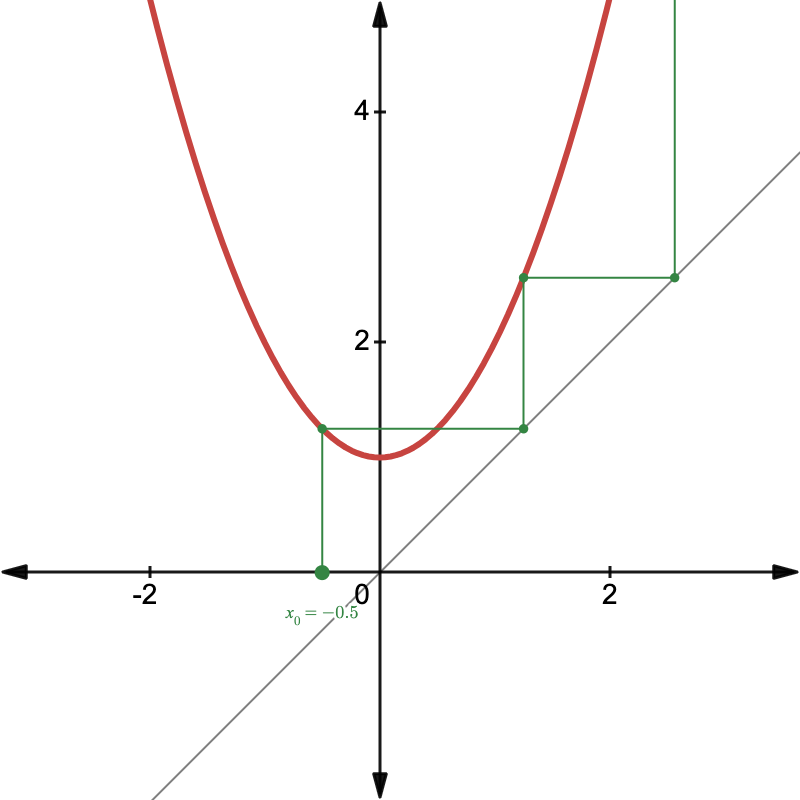
\includegraphics[width=6cm, height=4.5cm]{Grafi/cobweb1.png}
\end{centering}
\end{figure}

\newpage
Postopek:
\begin{itemize}
\item izbereš $x_0$ na osi $x$,
\item greš navpično na $f(x)$,
\item greš vodoravno do $y = x$,
\item ponavljaš zadnja dva koraka.
\end{itemize}
\end{primer}


\begin{primer}
Sherlock: $x_{n+1} = \frac{1}{2} x_n + \frac{5}{2}$ oz. $f(x) = \frac{1}{2} x + \frac{5}{2}$.\\ 

\begin{figure}[h]
    \begin{centering}
   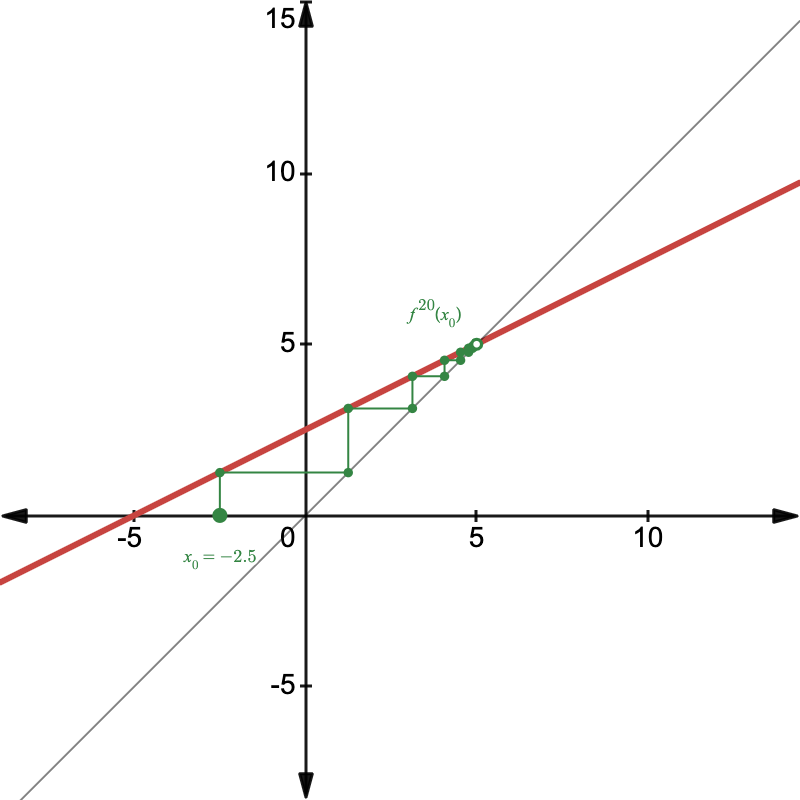
\includegraphics[width=6cm, height=5.5cm]{Grafi/cobweb2.png}
    \end{centering}
\end{figure}
    
$O_f(5) = \{5, 5, \dots \}$. Za ostale orbite velja: $x_n \rightarrow 5$.
\end{primer}

\begin{definicija}
Točka \textbf{$x_0 \in \R$ je periodična s periodo $n\in \N$} za $f$, če zanjo velja $f^n(x_0) = x_0$ in je $n$ najmanjše naravno število s to lastnostjo. Če je $n=1$, taki točki pravimo \textbf{fiksna točka}.
\end{definicija}

\begin{primer}
$f(x) = -x^3$. \\ 
Fiksne točke: 
$$f(x) = x \iff -x^3 = x \iff x = 0.$$ 
Točke periode $2$: $$f^2(x) = x \text{ in } f(x) \neq x \iff x^9 = x \text{ in } -x^3 \neq x\iff x = \pm 1.$$


\begin{figure}[h!]
    \begin{centering}
        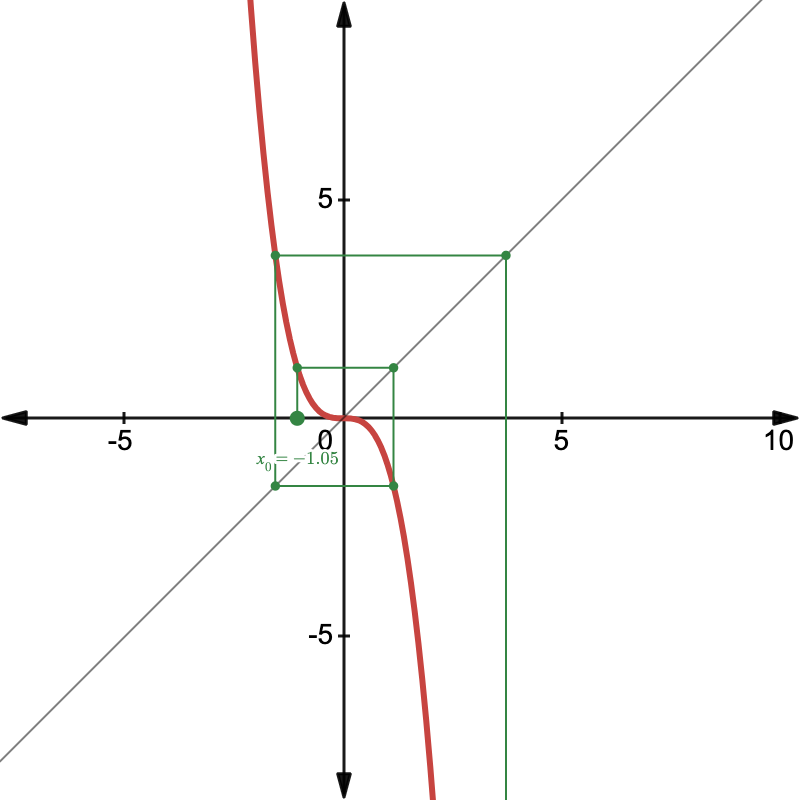
\includegraphics[width=6cm, height=5.5cm]{Grafi/cobweb3.png}
        \caption{pajčevinast diagram iz Primera 3.}
    \end{centering}
    \end{figure}    
\end{primer}

\begin{definicija}
Orbiti $n$- periodične točke rečemo $n$-cikel.
\end{definicija}

\newpage
\begin{definicija}
Naj bo $x_0 \in I$ fiksna točka za $f:I \rightarrow I$.
\begin{itemize}
\item $x_0$ je \textbf{šibko privlačna}, če obstaja njena okolica $U\subseteq I$, da za vsak $y_0 \in U$ velja $y_n = f^n(y_0) \rightarrow x_0$.
\item $x_0$ je \textbf{šibko odbojna}, če obstaja njena okolica $U\subseteq I$, da za vsak $y_0 \in U\backslash\{x_0\}$ obstaja $m\in \N$, da $f^m(x_0) \not\in U$.
\end{itemize}
Okolici iz prve točke pravimo \textbf{območje privlaka za $x_0$}, največjemu intervalu znotraj $U$, ki vsebuje $x_0$ pa rečemo \textbf{neposredno območje privlaka za $x_0$}.\\ 
\end{definicija}

\begin{opomba}
Če je $f \in C^0(I)$ in $f^n(x) \rightarrow x_0$ je $x_0$ nujno fiksna točka:
$$
f^n(x) \rightarrow x_0 \Longrightarrow \lim_{n\rightarrow \infty} f^{n+1}(x)= f(x_0) = x_0 = 
\lim_{n\rightarrow \infty} f^n(x)
$$
\end{opomba}

\begin{definicija}
Če je $f \in C^1(I)$, dodamo pojme:
\begin{itemize}
\item $x_0$ je \textbf{privlačna}, če $|f'(x_0)| < 1$.
\item $x_0$ je \textbf{odbojna}, če $|f'(x_0)| > 1$.
\item $x_0$ je \textbf{nevtralna}, če $|f'(x_0)| = 1$.
\end{itemize} 
\end{definicija}

\begin{primer}
Sherlock: $f(x) = \frac{1}{2}x + \frac{5}{2}$.
$f'(5) = \frac{1}{2}$ je privlačna in šibko privlačna.
\end{primer}

\newpage
\begin{primer}
Dane imamo tri funkcije $f_1(x) = x + x^3$, $f_2(x) = x - x^3$ in 
$f_3(x) = x + x^2$ 
    \begin{figure}[h]
        \centering
        % First figure
        \begin{subfigure}[b]{0.3\textwidth}
            \centering
            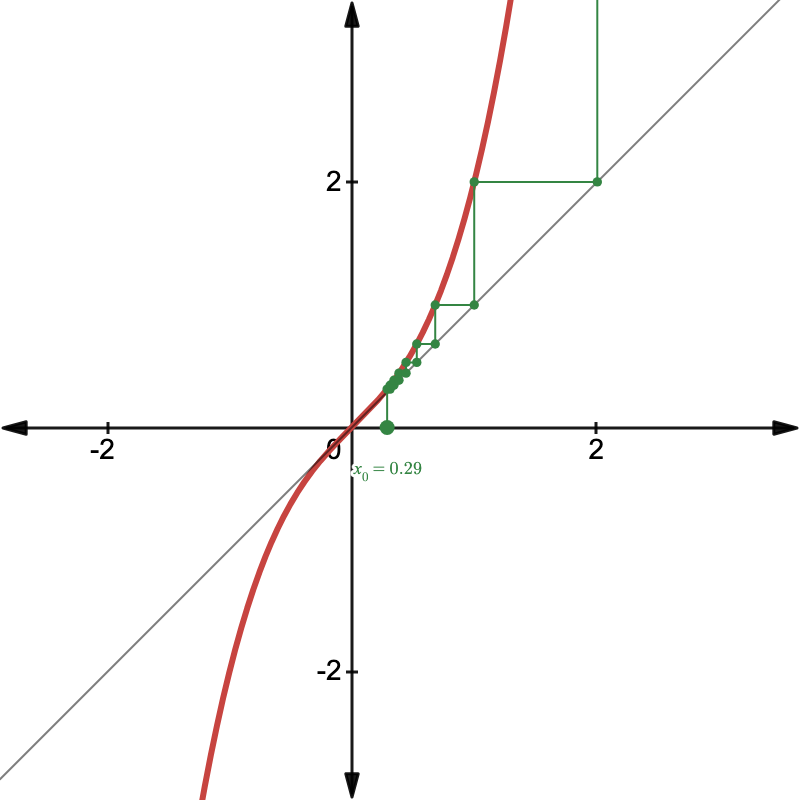
\includegraphics[width=\textwidth]{Grafi/cobweb41.png}
            \caption{\\$U = \R$\\$x=0$ šibko odbojna}
            \label{fig:cobweb31}
        \end{subfigure}
        % Second figure
        \begin{subfigure}[b]{0.3\textwidth}
            \centering
            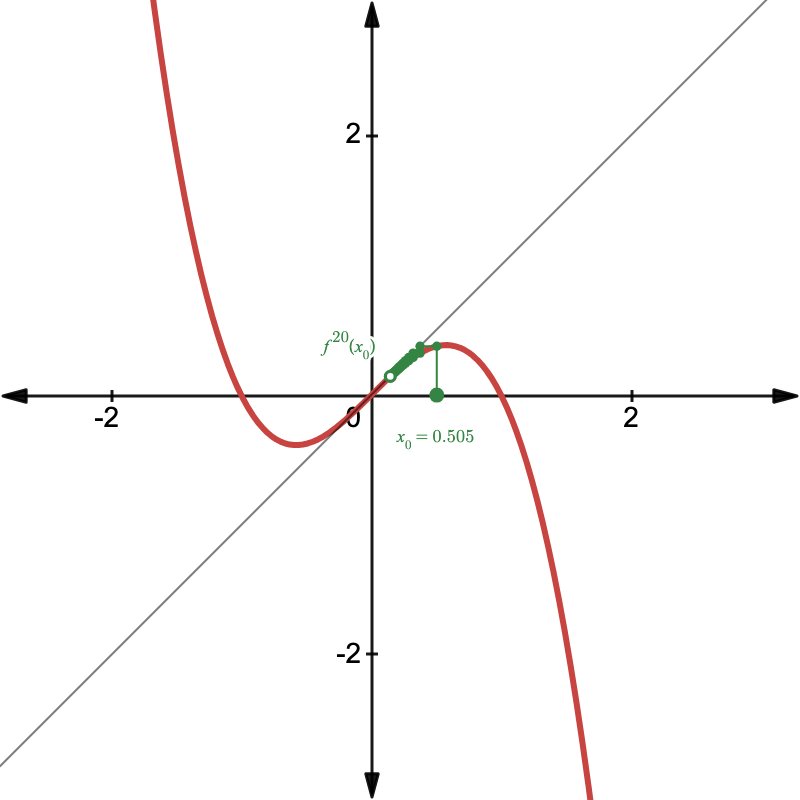
\includegraphics[width=\textwidth]{Grafi/cobweb42.png}
            \caption{\\$U = [-1,1]$\\$x=0$ šibko privlačna}
            \label{fig:cobweb32}
        \end{subfigure}
        % Third figure
        \begin{subfigure}[b]{0.3\textwidth}
            \centering
            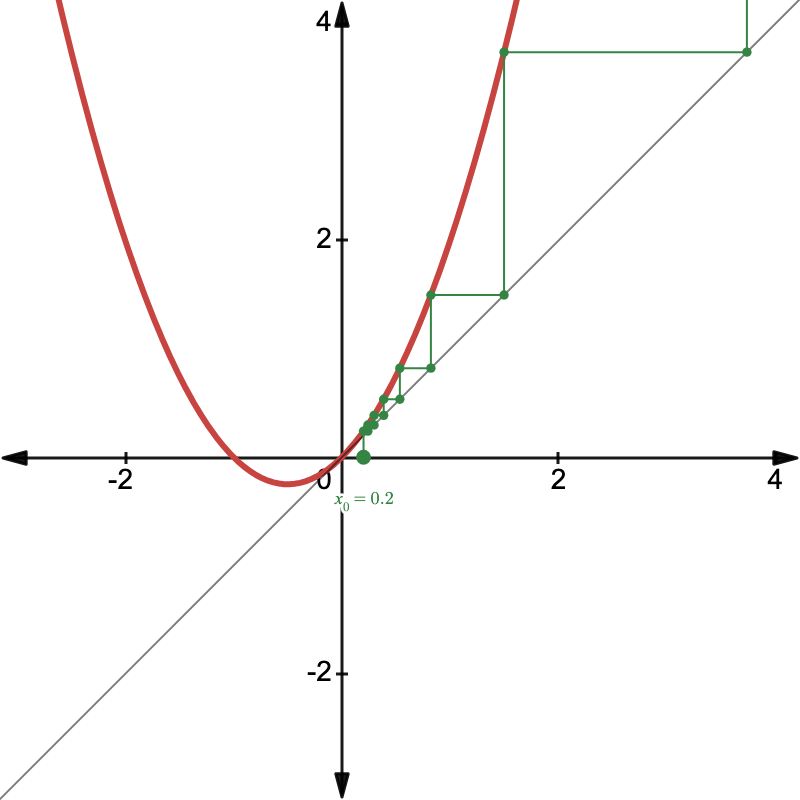
\includegraphics[width=\textwidth]{Grafi/cobweb43.png}
            \caption{\\$x=0$ ni šibko odbojna\\ ne privlačna}
            \label{fig:cobweb33}
        \end{subfigure}
    \end{figure}
V vseh treh primerih pa je $|f'(0)| = 1$ tj. gre za nevtralne točke.
\end{primer}

\begin{izrek}
Naj bo $f\in C^1(I)$ in $x_0 \in I$ fiksna točka. Potem velja:
\begin{enumerate}
\item[i)] Če je $|f'(x_0)| < 1$, je $x_0$ šibko privlačna.
\item[ii)] Če je $|f'(x_0)| > 1$, je $x_0$ šibko odbojna. 
\item[iii)] Če je $|f'(x_0)| = 1$, je $x_0$ nevtralna, pogledamo višje odvode za več informacij.
\end{enumerate}
\end{izrek}

\begin{proof}[Dokaz:]
\hfil
\begin{enumerate}
\item[i):] Recimo, da je $|f'(x_0)| < \lambda < 1$. Potem obstaja $\delta > 0$, da je $|f'(x_0)| < \lambda$ za vsak $x\in (x_0 - \delta, x_0 + \delta)$ zaradi zveznosti odvoda. Uporabimo Lagrangeov izrek
$$
f'(x) = \frac{f(x) - f(x_0)}{x - x_0} \quad \text{ za } c\in (x, x_0).
$$
Ker je $x_0$ fiksna točka
$$
f'(x) = \frac{f(x) - x_0}{x - x_0}.
$$
Naredimo oceno 
$$
|f(x) - x_0| = |f'(c)|\cdot |x - x_0| < \lambda |x - x_0|. 
$$
Zato za $x\in (x_0 - \delta, x_0 + \delta)$, velja da je tudi $f(x) \in (x_0 - \delta, x_0 + \delta)$. Indultivno sklepamo
$$
|f(f(x)) - f(x_0)| = |f^2(x) - x_0| < \lambda^2 |x - x_0|
$$
oz. 
$$
|f^n(x) - x_0| < \lambda^n |x - x_0|.
$$
Ker je $\lambda \in (0, 1)$, gre $\lambda^n \rightarrow 0$ za $n\rightarrow \infty$ torej $\lim_{n\rightarrow \infty} f^n(x) = x_0$.
\item[ii):] Dokaz je podoben, le da $\lambda > 1$ tj. za nek velik $m\in \N$, bo $\lambda^m |x - x_0|$ šel iz okolice.
\end{enumerate}
\end{proof}

\begin{definicija}
Fiksna točka $x_0 \in I$ je \textbf{stabilna} za $f:I \rightarrow I$, če za vsako njeno okolico $U \subset I$ obstaja manjša okolica $U' \subset U$, da za vsak $x\in U'$ velja $O_f(x) \subset U$.
\end{definicija}

\begin{opomba}
Iz dokaza izreka sledi, da privlačnost porodi enakomerno konvergenco 
$f^n(x) \rightarrow x_0$ za vse $x\in (x_0 - \delta, x + \delta)$.
Sledi, da so vse privlačne fiksne točke stabilne. 
Pa tudi take, katerih bližnje orbite ne konvergirajo nujno k $x_0$ tj. obstajajo 
nevtralne točke, ki niso šibko privlačne, a so vseeno stabilne npr. 
$f(x) = 1 - x$. Imamo $f^2(x) = x$ in $f(\frac{1}{2}) = \frac{1}{2}$ in 
$f'(\frac{1}{2}) = -1$. Torej je $\frac{1}{2}$ nevtralna fiksna točka, ostale 
točke so $2$-periodične. $x = \frac{1}{2}$ je stabilna.
\begin{figure}[h!]
    \begin{centering}
        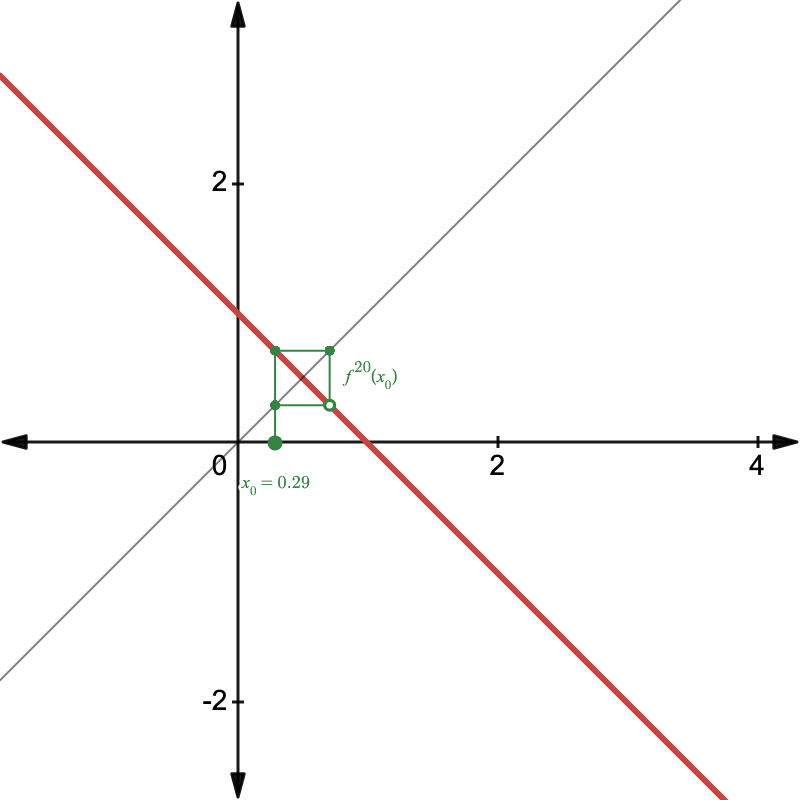
\includegraphics[width=6cm, height=5.5cm]{Grafi/cobweb5.png}
        %\caption{pajčevinast diagram iz Primera 3.}
    \end{centering}
    \end{figure}    
\end{opomba}

\begin{definicija}
Fiksne točke, ki so stabilne in šibko privlačne pravimo \textbf{asimptotsko stabilne}.
\end{definicija}

\begin{opomba}
Ni vsaka šibko privlačna točka (asimptotsko) stabilna. Orbita lahko "uide"
iz okolice in se nato vrne. So pa use privlačne točke tudi asimptotsko stabilne.
\end{opomba}

Sedaj lahko to klasifikacijo razširimo na $n$-periodične točke, če nanje pogledamo kot na fiksne točke funkcije $f^n$.
\begin{definicija}
Periodična točka $x_0 \in I$ oz. pripadajoči $n$-cikel je:
\begin{itemize}
\item Šibko privlačna\slash odbojna, če je šibko privlačna\slash odbojna kot fiksna točka funkcije $f^n$.
\item Privlačna\slash odbojna\slash nevtralna, če je privlačna\slash odbojna\slash nevtralna kot fiksna točka funkcije $f^n$. 
\end{itemize}
\end{definicija}
Da bosta ti definiciji dobri, v prvi točki potrebujemo zveznost, v drugi pa zvezno odvedljivost funkcije $f$. To združi nasledji izrek.
\begin{izrek}
Če je $f\in C^1(I)$, so vse periodične točke $n$-cikla "istega tipa".
\end{izrek}

\begin{proof}[Dokaz:]
Naj bo $\{x_1, \dots, x_n\}$ $n$-cikel za $f$. Recimo, da je $x_n$ šibko privlačna 
za $f^n$. Torej obstaja njena okolica $U_n \subset I$, da za 
$x\in U_n$ velja $f^{nk}(x) \rightarrow x_n$ za $k\rightarrow \infty$. 
Radi bi videli, da analogne okolice obstajajo za točke 
$x_1, \dots, x_{n-1}$. Sedaj definiramo $U_{n-j}$ za $1 \leq j \leq n-1$, 
kot povezano komponento praslike $f^{-j}(U_n)$, ki vsenuje $x_{n-j}$. Vemo,
da za vsak $x\in U_{n-j}$ po konstrukciji velja:
$$
f^{nk + j}(x) \xrightarrow{k\rightarrow \infty} x_n.
$$
Sedaj na to zvezo dodamo zvezno funkcijo $f^{n-j}$
\begin{align*}
f^{n-j}(f^{nk + j}(x)) \rightarrow f^{n-j}(x_n) \\ 
f^{n(k+1)}(x) \xrightarrow{k\rightarrow \infty} x_{n-j} 
\end{align*}
vse točke so šibko privlačne, kar smo želeli dokazati. Dokaz za šibko odbojnost izpustimo.\\[3mm]
Poglejmo si še privlačnosti\slash odbojnost \slash nevtralnost
\begin{align*}
|(f^n)'(x_n)| &= |(f \circ f \circ \dots \circ f)'(x_n)| = \\ 
&= |f'(f^{n-1}(x_n)) \cdot f'(f^{n-2}(x_n)) \cdot \dots f'(x_n)| = \\ 
&= |f'(x_{n-1})| \cdot |f'(x_{n-2})| \cdot \dots |f'(x_1)| \cdot |f'(x_0)| = |(f^n)'(x_j)|.
\end{align*}
za vsak $x_j$ dobimo isti rezultat.
\end{proof}

\begin{opomba}
Brez zveznosti $f$ izrek ne drži nujno, npr.
\begin{centering}
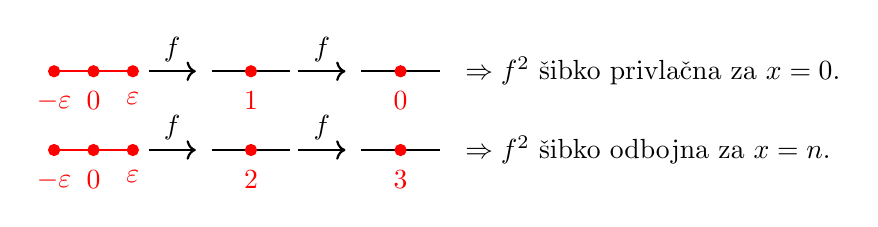
\begin{tikzpicture}[scale=1]

    % First line (maps to 1, then to 0)
    % Left interval (shorter but aligned)
    \draw[thick] (-3.5,1.5) -- (-2.5,1.5);
    \draw[red, thick] (-3.5,1.5) -- (-2.5,1.5);
    
    % epsilon points and zero point
    \filldraw[red] (-3.5,1.5) circle (2pt) node[below=4pt] {$-\varepsilon$};
    \filldraw[red] (-2.5,1.5) circle (2pt) node[below=4pt] {$\varepsilon$};
    \filldraw[red] (-3,1.5) circle (2pt) node[below=4pt] {$0$};
    
    % Short arrow to 1 with more space
    \draw[->, thick] (-2.3,1.5) -- (-1.7,1.5);
    \node[above] at (-2,1.5) {$f$};
    
    % Longer interval at 1 with more space from the arrow
    \draw[thick] (-1.5,1.5) -- (-0.5,1.5);
    \filldraw[red] (-1,1.5) circle (2pt) node[below=4pt] {$1$};
    
    % Short arrow to 0 with more space
    \draw[->, thick] (-0.4,1.5) -- (0.2,1.5);
    \node[above] at (-0.1,1.5) {$f$};
    
    % Longer interval at 0 with more space from the arrow
    \draw[thick] (0.4,1.5) -- (1.4,1.5);
    \filldraw[red] (0.9,1.5) circle (2pt) node[below=4pt] {$0$};
    
    % Comment
    \node[right] at (1.6,1.5) {$\Rightarrow f^2$ šibko privlačna za $x=0$.};
    
    % Second line (maps to 2, then to 3)
    % Left interval (shorter but aligned)
    \draw[thick] (-3.5,0.5) -- (-2.5,0.5);
    \draw[red, thick] (-3.5,0.5) -- (-2.5,0.5);
    
    % epsilon points and zero point
    \filldraw[red] (-3.5,0.5) circle (2pt) node[below=4pt] {$-\varepsilon$};
    \filldraw[red] (-2.5,0.5) circle (2pt) node[below=4pt] {$\varepsilon$};
    \filldraw[red] (-3,0.5) circle (2pt) node[below=4pt] {$0$};
    
    % Short arrow to 2 with more space
    \draw[->, thick] (-2.3,0.5) -- (-1.7,0.5);
    \node[above] at (-2,0.5) {$f$};
    
    % Longer interval at 2 with more space from the arrow
    \draw[thick] (-1.5,0.5) -- (-0.5,0.5);
    \filldraw[red] (-1,0.5) circle (2pt) node[below=4pt] {$2$};
    
    % Short arrow to 3 with more space
    \draw[->, thick] (-0.4,0.5) -- (0.2,0.5);
    \node[above] at (-0.1,0.5) {$f$};
    
    % Longer interval at 3 with more space from the arrow
    \draw[thick] (0.4,0.5) -- (1.4,0.5);
    \filldraw[red] (0.9,0.5) circle (2pt) node[below=4pt] {$3$};
    
    % Comment
    \node[right] at (1.6,0.5) {$\Rightarrow f^2$ šibko odbojna za $x=n$.};
    
\end{tikzpicture}
\end{centering}
\end{opomba}

\newpage

\begin{primer}
Dano imamo $f(x) = x^2 - 1$. Opazimo $f(0) = -1$ in $f(-1) = 0$ tj. imamo $2$-cikel. Poglejmo, katarega tipa je:
$$
(f^2)'(0) = f'(f(0)) \cdot f'(0) = f'(-1)\cdot f'(0) = 0.
$$
Torej gre za privlačen $2$-cikel. Fiksni točki sta $x = \frac{1 \pm \sqrt{5}}{2}$
$\Longrightarrow$ $f'\Big(\frac{1 \pm \sqrt{5}}{2}\Big) = 1 \pm \sqrt{5}$, torej 
sta obe odbojni.
\begin{figure}[h!]
    \begin{centering}
        
    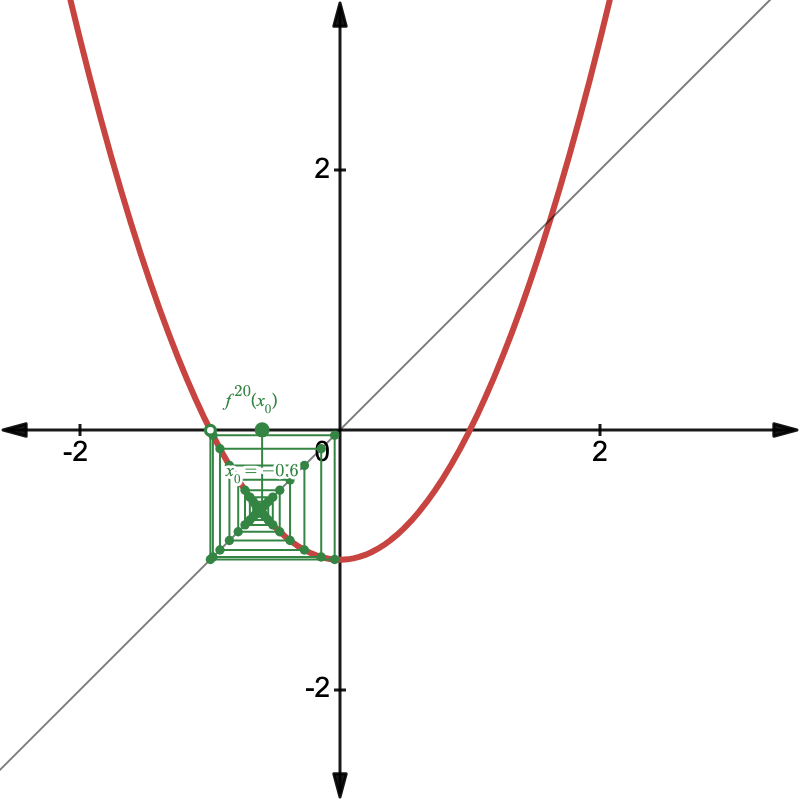
\includegraphics[width=6cm, height=5.5cm]{Grafi/cobweb6.png}
    %\caption{pajčevinast diagram iz Primera 3.}
    \end{centering}
\end{figure}    
\noindent
Vidimo, da $2$-cikel "privlači" bližnje orbite. To velja tudiv primeru 
šibke privlačnosti. Naj bosta $U_1$ in $U_2$ okolici točke $x_1$ in $x_2$,
ki pripadata $2$-ciklu. Vzamemo $\tilde{U}_1 = U_1\cap f^{-1}(U_2)$ in 
$\tilde{U}_2 = U_1\cap f^{-1}(U_1)$. Potem velja:
\begin{align*}
x\in \tilde{U}_1 \Longrightarrow f^{2n}(x) \rightarrow x_1 \,\,(\text{ker } x\in U_1)\,\, \text{ in }\,\, f^{2n+1}(x) \rightarrow x_2 \,\,(\text{ker } f(x)\in U_2)\\
x\in \tilde{U}_2 \Longrightarrow f^{2n}(x) \rightarrow x_2 \,\,(\text{ker } x\in U_2)\,\, \text{ in }\,\, f^{2n+1}(x) \rightarrow x_1 \,\,(\text{ker } f(x)\in U_1)
\end{align*}


\begin{opomba}
Zanimiva je tudi točka $x = 1$, ki ima orbito $O_f(1) = \{1, 0, -1, 0, -1, \dots\}$ 
tj. po prvi iteraciji postane ciklična. Takim točkam pravimo \textbf{predperiodična} 
(preperiodic \slash eventually periodic) točka.
\end{opomba}
\end{primer}

\begin{definicija}
$\exists k\in \N$: $f^{n+k}(x) = f^k(x)$ za  najmanjši tak $n\in \N$.
\end{definicija}

\section{Kaos}
Do sedaj smo spoznali le dinamične sisteme z razmeroma predvidljivim dogajanjem. Konkretno, razen v kakšni posebni točki, so imele orbite bližnjih točk "enak dinamičen razvoj". Sedaj bomo spoznali sisteme, ki so nasprotje tega in jim pravimo kaotični. 

\begin{definicija}[Devaney]
Dinamični sistem podan z $f:I \rightarrow I$ je \textbf{kaotičen}, če zanj veljajo
\item[(c1)] Množica periodičnih točk je gosta v $I$.
\item[(c2)] Tranzitivnost: za poljubna odprta intervala $U_1, U_2 \subset I$, obstajata $x_0\in U_1$ in $n\in \N$, da je $f^n(x_0) \in U_2$.
\item[(c3)] Občutljivostna konstanta: obstaja $\beta > 0$, da v poljubni okolici $U$ poljubne točke $x_0$ najdemo tudi točko $y_0 \in U$ za katero je $|f^n(x_0) - f^n(y_0)| > \beta$ za nek $n\in \N$.
\end{definicija}

\begin{opomba}
\hfill 
\begin{itemize}
\item Točka $(c3)$ je zanimiva pri izbiri majhnih okolic $U$, saj pomeni, da lahko poljubno blizu najdeš točko s čisto drugačno dinamiko. Temu se reče učinek metulja (butterly effect) tj. zaporedje oz. orbita je občutljiva na začetne podatke.
\item Izkaže se, da je $(c2)$ ekvivalentna obstoju goste orbite, če je $f$ zvezna. Če ni zvezna je pogoj zadosten.
\item Za kompakt $I \subset I$ se izkaže, da $(c1)$ in $(c2)$ implicirata $(c3)$.
\item Če je $f$ zvezna iz $(c1)$ in $(c2)$ vedno sledi $(c3)$.
\end{itemize}
\end{opomba}
\noindent
Opis kaosa: kaotični sistem je tak, v katerem s približnim začetkom niti približno nemoreš napovedati konca.

\begin{primer}
Podvojitvena preslikava (doubling map).
\begin{align*}
D:[0, 1) \rightarrow [0, 1) \\ 
D(x) = 2x - \lfloor{2x}\rfloor
\end{align*}
\begin{figure}[h!]
    \begin{centering}
        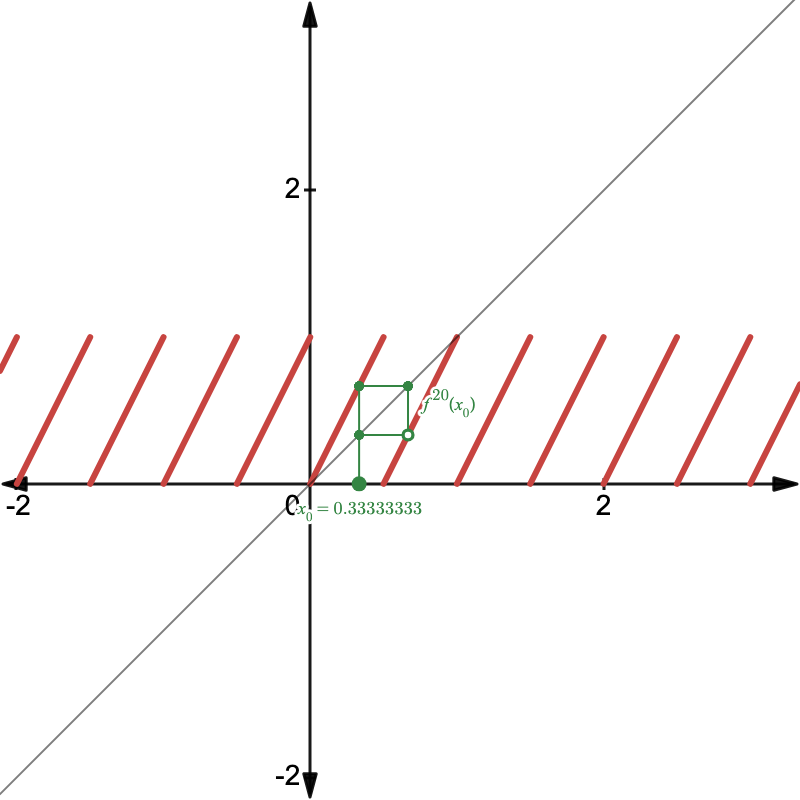
\includegraphics[width=6cm, height=5.5cm]{Grafi/cobweb7.png}
        %\caption{pajčevinast diagram iz Primera 3.}
    \end{centering}
\end{figure}   
\noindent
Velja: \\ 
$D(0) = 0$ je fiksna točka \\ 
$D(\frac{1}{2}) = 0$ predperiodična \\ 
$D(\frac{1}{3}) = \frac{2}{3}$, $D(\frac{2}{3}) = \frac{1}{3}$ 2-cikel.\\
Za dokaz kaotičnosti uporabimo dvojiški decimalni zapis.
\begin{align*}
x\in [0, 1): x = 0.x_1 x_2 \dots_{(2)} = \sum_{j=1}^\infty \frac{x_j}{2^j}, \quad x_j\in \{0, 1\}
\end{align*}
Če prepovemo neskočen niz enic, je zapis enoličen. Kaj naredi naša preslikava?
\begin{align*}
D(x) = 2x - \lfloor 2x \rfloor = x_1.x_2 x_3 \dots_{(2)} - {x_1}_{(2)} = 0.x_2 x_3 \dots_{(2)}.
\end{align*}
Temu rečemo tudi operator zamika (shift map), ki "pozabi" prvo decimalko. 
\begin{enumerate}
\item[(c1)] Pokažimo, da imamo poljubno blizu točke $x\in [0, 1)$ tudi periodično točko $\tilde{x}$.
\begin{align*}
x &= 0.x_1 x_2 \dots x_N x_{N+1} \dots_{(2)} \quad N >> 1 \\ 
\tilde{x} &= 0.\overline{x_1 x_2 \dots x_N}_{(2)}\\
\Longrightarrow& |x - \tilde{x}| = 0.0\dots 0x_{N+1}\dots_{(2)} < \frac{1}{2^N}
\end{align*}
Očitno je $\tilde{x}$ periodičen, saj je $f^N(\tilde{x}) = \tilde{x}$. Po drugo strani pa je $|x - \tilde{x}| < \frac{1}{2^N}$ tj. poljubno majhna.
\item[c2)] Pokažimo, da obstaja gosta orbita. Naj bo $x\in [0, 1]$ število z razvojem
$$
x = 0.01\, 00\, 01\, 10\, 11\, 000\, 001\, 010\, \dots
$$
tj. število vsebuje vse končne zapise v dvojiškem sistemu. Trdimo, da je 
za vsak $x\in [0, 1]$ blizu nek $D^m(\tilde{x})$. 
$$
x = 0.x_1 x_2\dots x_N x_{N+1}\dots, \quad \text{ za } N>>1.
$$
Obstaja tak $m\in \N: f^m(x) = 0.x_1 x_2 \dots x_N y_{N+1}$ tj. $|f^m(\tilde{x}) - x| < \frac{1}{2^N}$.
\item[c3)] Želimo videti, da poljubno blizu $x\in [0, 1]$ obstaja $\tilde{x} \in [0, 1]$, da je za nek $m\in \N$: $|f^m(x) - f^m(\tilde{x}) \geq \frac{1}{2}$. 
Vzamemo
$$
x = 0.x_1 x_2 \dots x_N x_{N+1} \dots_{(2)}
$$
in
$$
\tilde{x} = 0.\tilde{x}_1 \tilde{x}_2\dots \tilde{x}_N \tilde{x}_{N+1} \dots_{(2)}
$$
Naj velja $\tilde{x}_{N+1} \neq x_{N+1}$
Potem je 
$$
|f^N(x) - f^N(\tilde{x})| = |0.x_{N+1}x_{N+2}\dots  - 0.\tilde{x}_{N+1} \tilde{x}_{N+2}\dots| \geq \frac{1}{2}.
$$
Dobimo števili, ki sta $\frac{1}{2^N}$ blizu in po $n$-iteracijah $\frac{1}{2}$ narazen.
\end{enumerate}
\end{primer}
\newpage
\begin{primer}
Šotorasta preslikava(Tent map)
$$
T(x)= \begin{cases}2 x ; & x \in\left[0, \frac{1}{2}\right] \\ 2-2 x ; & x \in\left(\frac{1}{2}, 1\right]\end{cases} =2\min\{x, 1 - x\} 
$$
\begin{figure}[h!]
    \begin{centering}
        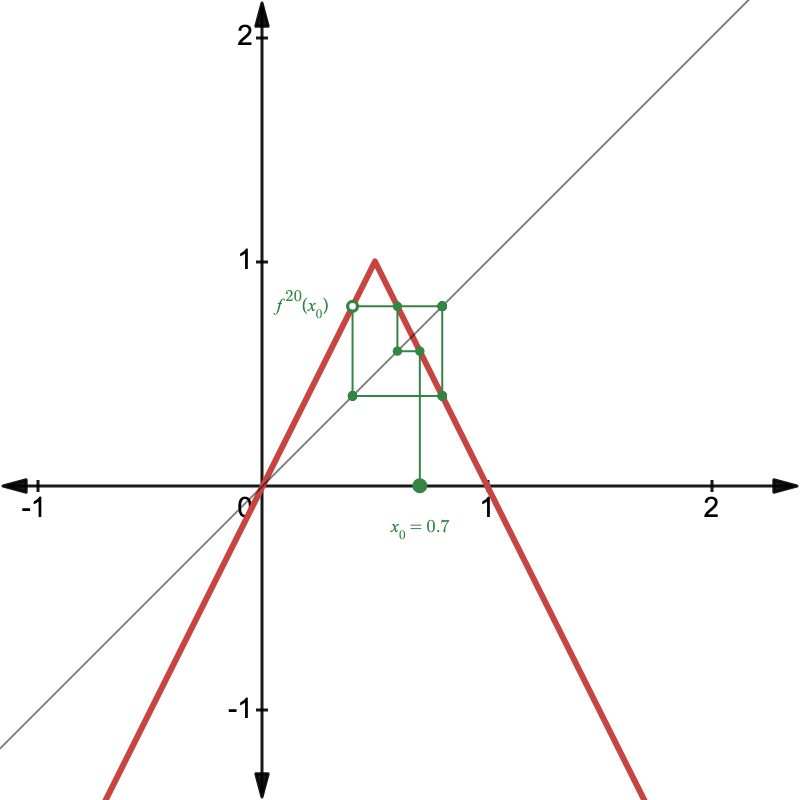
\includegraphics[width=6cm, height=5.5cm]{Grafi/cobweb8.png}
    %\caption{paj čevinast diagram iz Primera 3.}
    \end{centering}
\end{figure}   

Drugi iterat: 
$$T^2(x) = \min\{T(x), 1 - T(x)\}$$

\begin{figure}[h!]
    \begin{centering}
        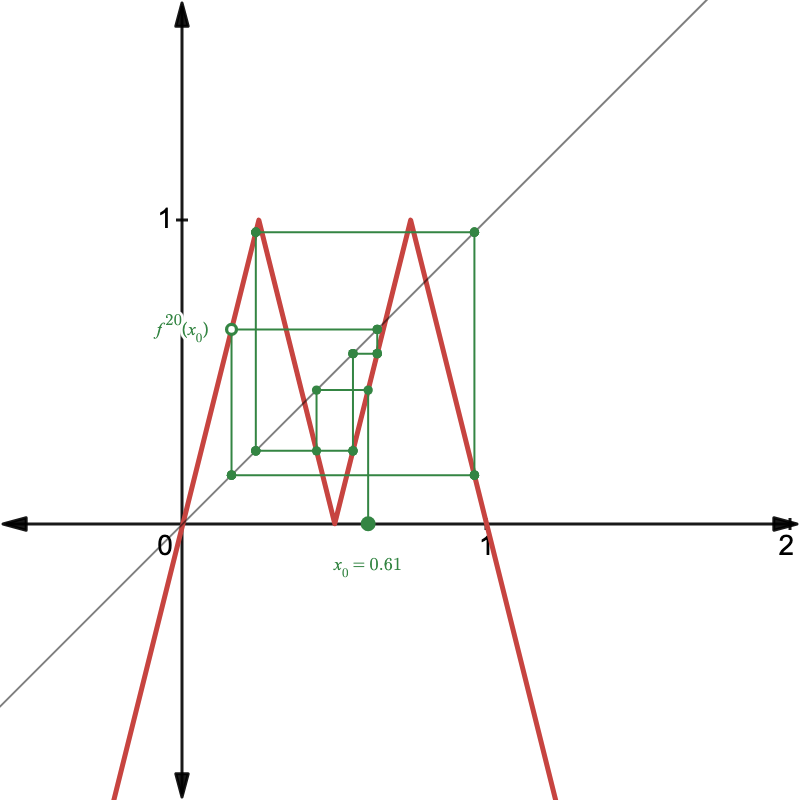
\includegraphics[width=6cm, height=5.5cm]{Grafi/cobweb9.png}
        %\caption{pajčevinast diagram iz Primera 3.}
    \end{centering}
\end{figure} 
\newpage
Podobno dobimo $T^3$ in višje iterate 

\begin{figure}[h!]
    \begin{centering}
        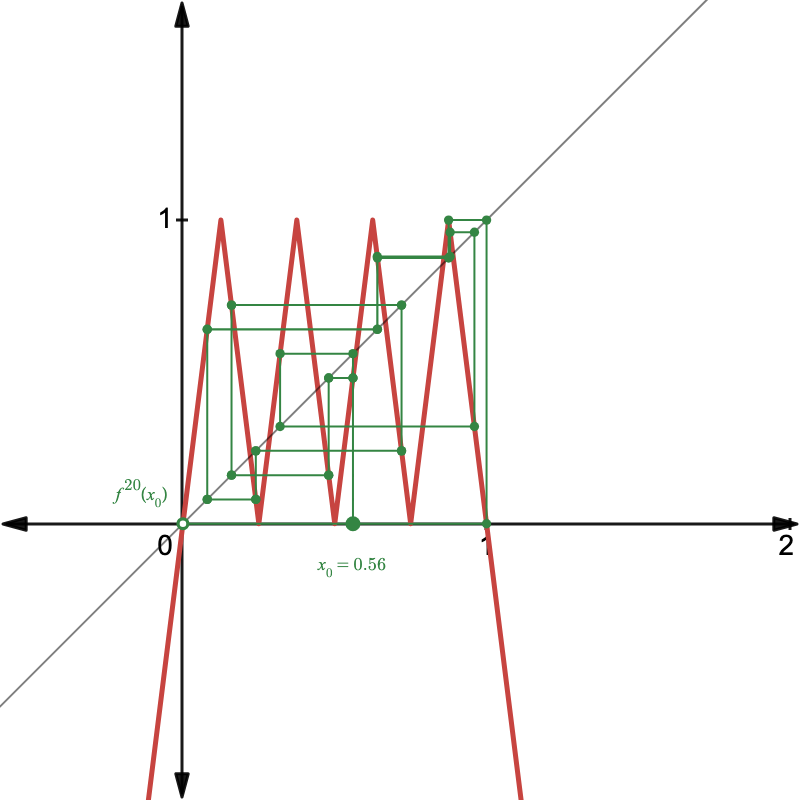
\includegraphics[width=6cm, height=5.5cm]{Grafi/cobweb10.png}
        %\caption{pajčevinast diagram iz Primera 3.}
    \end{centering}
\end{figure} 


Definiramo intervale 
$$
I_{j, n} \coloneqq \Big[\frac{j-1}{2^n}, \frac{j}{2^n}\Big], \quad j = \{1, 2, \dots, 2^n\}.
$$

\begin{enumerate}
\item[c1)] Je izpolnjen, saj ima periodično točko na vsakem intervalu oblike $I_{k, j}$.
Perioda teh točk je $n$ ali manjša.
\item[ii)] Sledi, ker je $f^n(I_{j,n}) = [0, 1]$, tj.
za $U_1$ obstaja $I_{j, n} \subset U_1$, bo $T(I_{j, n}) \cap U_2 \neq \emptyset$ za poljubni odprti $U_1, U_2 \subset [0, 1]$.
\item[c3)] Samo ideja: za vsak $x\in [0, 1]$, poiščemo $j, k$ in $\tilde{x} \in I_{j, n}$, 
da bo $T^k(x) - T^k(\tilde{x})| \geq \frac{1}{2}$.
\end{enumerate}
\end{primer}

\section{Konjugacije in semi-konjugacije}

\begin{definicija}
Pravimo, da sta $f: I \rightarrow I$ in $g: J \rightarrow J$ \textbf{konjugirani}, če obstaja homeomorfizem $h:I \rightarrow J$, da $\forall x\in I$: $h \circ f(x) = g\circ h(x) $
\end{definicija}
Imamo komutirajoči diagram za dano definicijo
\begin{centering}
\begin{tikzcd}
	I && I \\
	\\
	J && J
	\arrow["f", from=1-1, to=1-3]
	\arrow["h"', from=1-1, to=3-1]
	\arrow["h"', from=1-3, to=3-3]
	\arrow["g", from=3-1, to=3-3]
\end{tikzcd}
\end{centering}

Iz definicije sledi, da je $h(O_f(x)) = O_g(h(x))$ za vsak $x\in I$. Z drugimi 
besedami orbite $f$ se slikajo v orbite $h$ za $g$. To vodimo iz naslednjega razmisleka: 
ker je $h$ obrljiva in $h^{-1}$ zvezna, se zvezno traslira celotna dinamika tj.
\begin{align*}
f &= h^{-1} \circ g \circ h \Longrightarrow\\ 
f^n &= (h^{-1} \circ g \circ h) \circ (h^{-1} \circ g \circ h) \circ \dots \circ (h^{-1} \circ g \circ h) = \\ 
&= h^{-1} \circ g^n \circ h
\end{align*}

\begin{primer}
\begin{align*}
&g(x) = x^2 \text{ na } [0, \infty) \\ 
&f(x) = x^2 - 2x + 2 \text{ na } [1, \infty) \\ 
&h(x) = x - 1 \text{ kot preslikava } h:[1, \infty) \rightarrow [0, \infty).
\end{align*}
Preverimo pogoj iz definicije 
\begin{align*}
h\circ f(x) &= h(x^2 - 2x + 2) = x^2 -2x + 2 - 1 = x^2 - 2x - 1 = \\ 
&=(x-1)^2 = g(x-1) = g\circ h(x)  
\end{align*}

\begin{center}
    \begin{figure}[h]
        \centering
        \begin{subfigure}{0.45\textwidth}
            \centering
            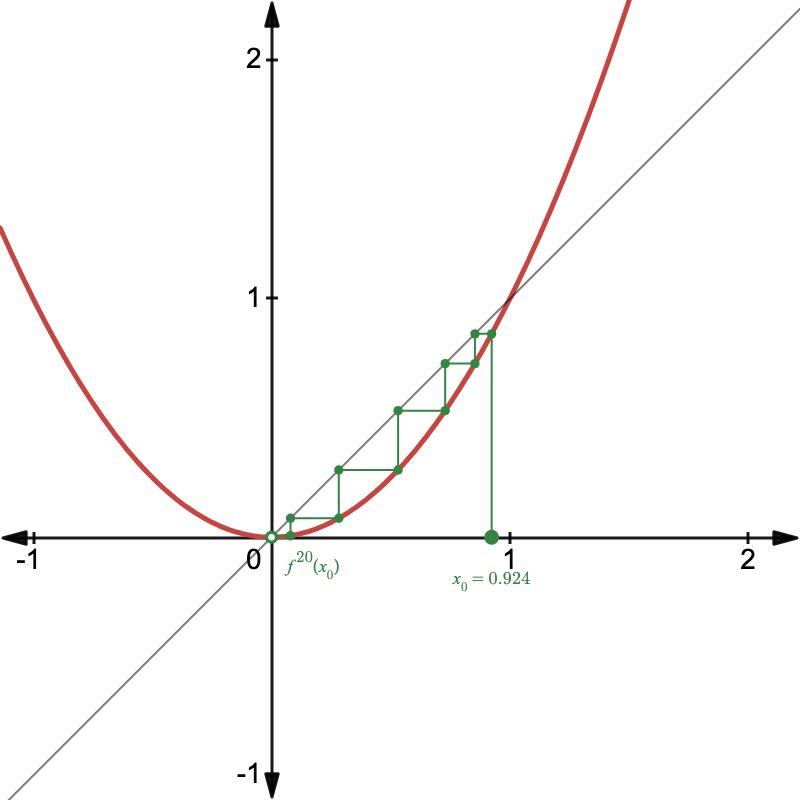
\includegraphics[width=\textwidth]{Grafi/cobweb11.png}
            \caption{$g(x) = x^2$}
        \end{subfigure}
        \hfill
        \begin{subfigure}{0.45\textwidth}
            \centering
            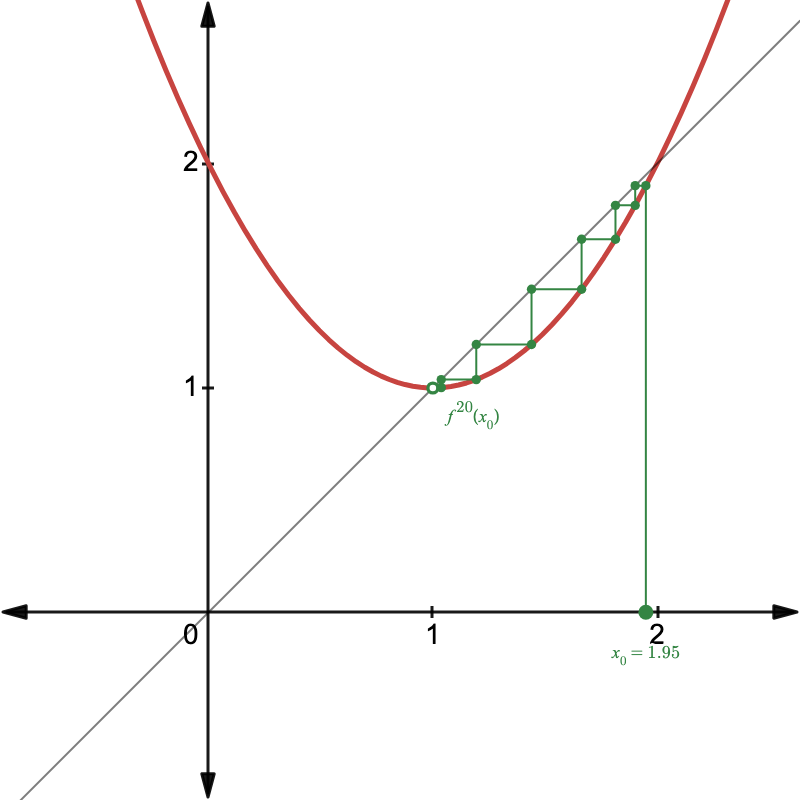
\includegraphics[width=\textwidth]{Grafi/cobweb12.png}
            \caption{$f(x) = x^2 - 2x + 2$}
        \end{subfigure}
        %\caption{Two images displayed side by side}
    \end{figure}
    
\end{center}
\end{primer}

\begin{opomba}
    \hfill
\begin{itemize}
\item V splošnem velja, da je vsaka kvadratna funkcija $f(x) = Ax^2+ Bx + C$, $A \neq 0$ konjugirana $p_c(x) = x^2 + c$, $c\in \R$.
\item Vidimo, da se je v primeru ohranil tudi karakter fiksnih točk. To ne preseneča oz. še več, če sta $h$ in $h^{-1}$ tudi odvedljivi, velja:
\begin{align*}
f'(x) &= (h^{-1} \circ g \circ h)(x) = (h^{-1}) (g(h(x))) \cdot g'(h(x)) \cdot h'(x) = \\ 
&= \frac{1}{h'(h^{-1} (g(h(x))))} \cdot g'(h(x))\cdot h'(x) = g'(h(x)),
\end{align*}
kjer smo uporabili dejstvo, da je $g(h(x)) = h(x)$ za fiksno točko $x$.
Torej se tip fiksne točke ograni. Podobno velja za periodične točke.
\end{itemize}
\end{opomba}

\begin{definicija}
Pravimo, da je $g: J \rightarrow J$ \textbf{semi-konjugirana} funkciji $f: I \rightarrow I$, če obstaja zvezna surjektivna preslikava $h:I \rightarrow J$, za katero velja:
\begin{enumerate}
\item[i)] $\forall x\in I$: $h\circ f(x) = g\circ h(x)$
\item[ii)] $\exists m\in \N.\, \forall x\in J$ ima $h^{-1}(x)$ največ $m$ elementov.
\end{enumerate}
\end{definicija}


\begin{center}
    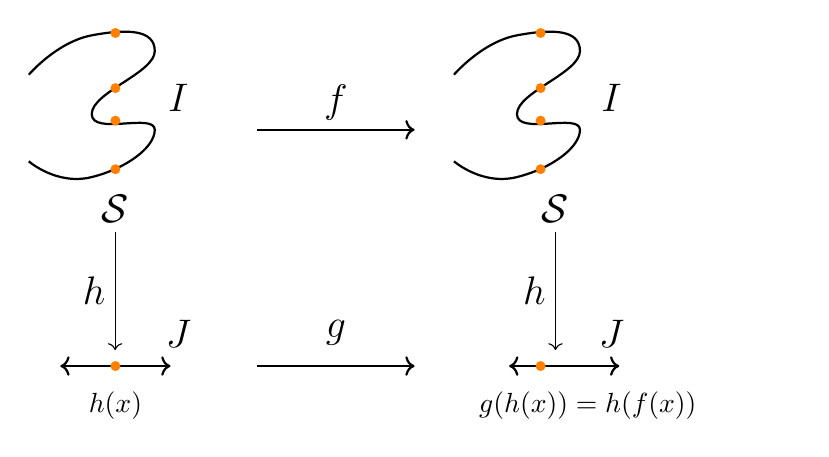
\begin{tikzpicture}[node distance=3cm, auto]
        % Nodes
        \node (S1) [right=4mm]{\Large $\mathcal{S}$};
        \node (I1) [right of=S1] {};
        \node (Z1) [below=15mm of S1] {};
        \node (S2) [right=50mm of S1] {\Large $\mathcal{S}$};
        \node (I2) [right of=S2] {};
        \node (Z2) [below=15mm of S2] {};
        
        \draw[thick][<->] (0,-2) -- (1.4,-2);
        \draw[thick][<->] (5.7,-2) -- (7.1,-2);  
        
        \draw[thick][->] (2.5,1) -- (4.5,1);
        \fill (3.5,1.7) node[below] {\Large$f$};

        \draw[thick][->] (2.5,-2) -- (4.5,-2);
        \fill (3.5,-1.3) node[below] {\Large$g$};

        \fill[orange] (0.7,-2) circle (1.8pt);
        \fill (0.7,-2.2) node[below] {$h(x)$};

        \fill[orange] (6.1,-2) circle (1.8pt);
        \fill (6.7,-2.2) node[below] {$g(h(x)) = h(f(x))$};

        \fill (7,1.7) node[below] {\Large $I$};
        \fill (1.5,1.7) node[below] {\Large $I$};

        \fill (7,-1.3) node[below] {\Large $J$};
        \fill (1.5,-1.3) node[below] {\Large $J$};

        % Arrows
        \draw[->] (S1) -- node[left] {\Large $h$} (Z1);
        %\draw[->] (I1) -- node[above] {\Large $F$} (I2);
        \draw[->] (S2) -- node[left] {\Large $h$} (Z2);
        %\draw[->] (Z1) -- node[below] {\Large $g$} (Z2);
    
    \draw[thick] plot [smooth, tension=1] coordinates 
        {(-0.4,1.7) (0.4,2.2) (1.2,2) (0.4,1.2) (1.2,1) (0.4,0.4) (-0.4,0.6)};
        
    \draw[thick] plot [smooth, tension=1] coordinates 
        {(5,1.7) (5.8,2.2) (6.6,2) (5.8,1.2) (6.6,1) (5.8,0.4) (5,0.6)};
    
    % Orange Points
    \foreach \x in {(0.7,2.23), (0.7,1.53), (0.7,1.117), (0.7,0.5)}
        \fill[orange] \x circle (1.8pt);
    
    \foreach \x in {(6.1,2.23), (6.1,1.53), (6.1,1.117), (6.1,0.5)}
        \fill[orange] \x circle (1.8pt);
        
    \end{tikzpicture}
    \end{center}

\begin{opomba}
\hfill
\begin{itemize}
    \item Definicija semi-konjugacije lahko varira glede na literaturo.
    \item Znova velja 
    $$
    h(O_f(x)) = O_g(h(x))
    $$
    vendar pa ta relacija ni več bijektivna.
\end{itemize}
\end{opomba}

\begin{primer}
Dane imamo naslednje preslikave 
\begin{figure}[h]
    \centering
    % First figure
    \begin{subfigure}[b]{0.32\textwidth}
        \centering
        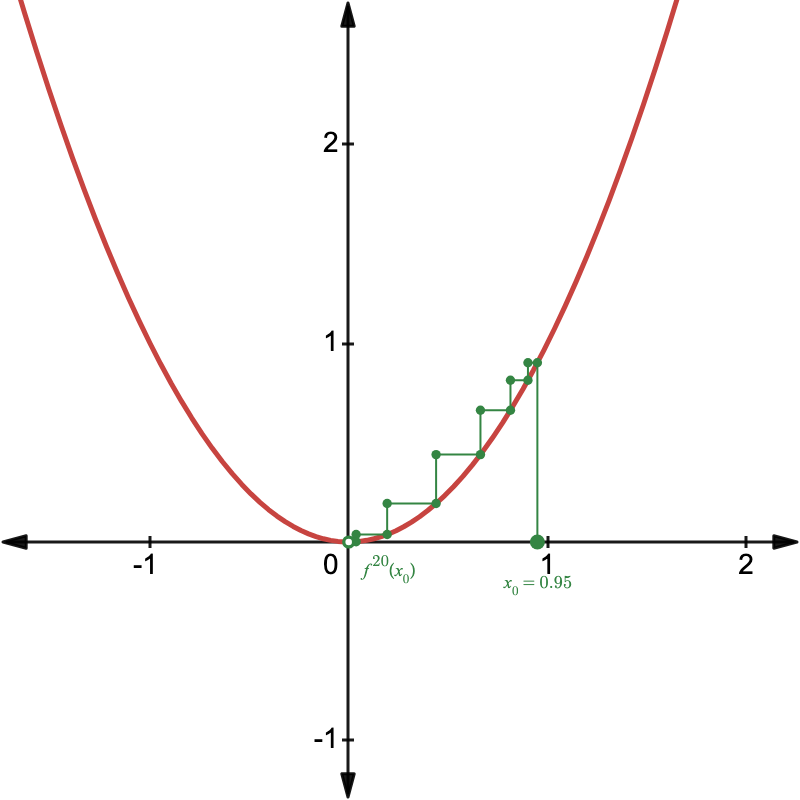
\includegraphics[width=\textwidth]{Grafi/cobweb131.png}
        \caption{\\$h:[-1, 1] \rightarrow [0, 1] $\\\quad $x \mapsto x^2$}
        \label{fig:cobweb31}
    \end{subfigure}
    % Second figure
    \begin{subfigure}[b]{0.32\textwidth}
        \centering
        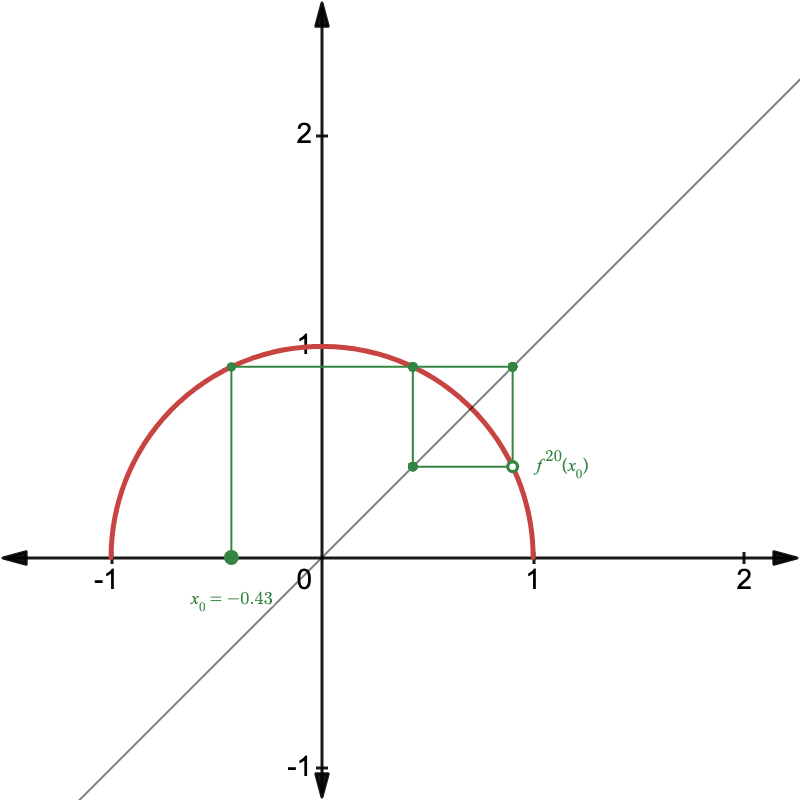
\includegraphics[width=\textwidth]{Grafi/cobweb132.png}
        \caption{\\$f:[-1, 1] \rightarrow [-1, 1]$ \\ $x\mapsto \sqrt{1 - x^2}$}
        \label{fig:cobweb32}
    \end{subfigure}
    % Third figure
    \begin{subfigure}[b]{0.32\textwidth}
        \centering
        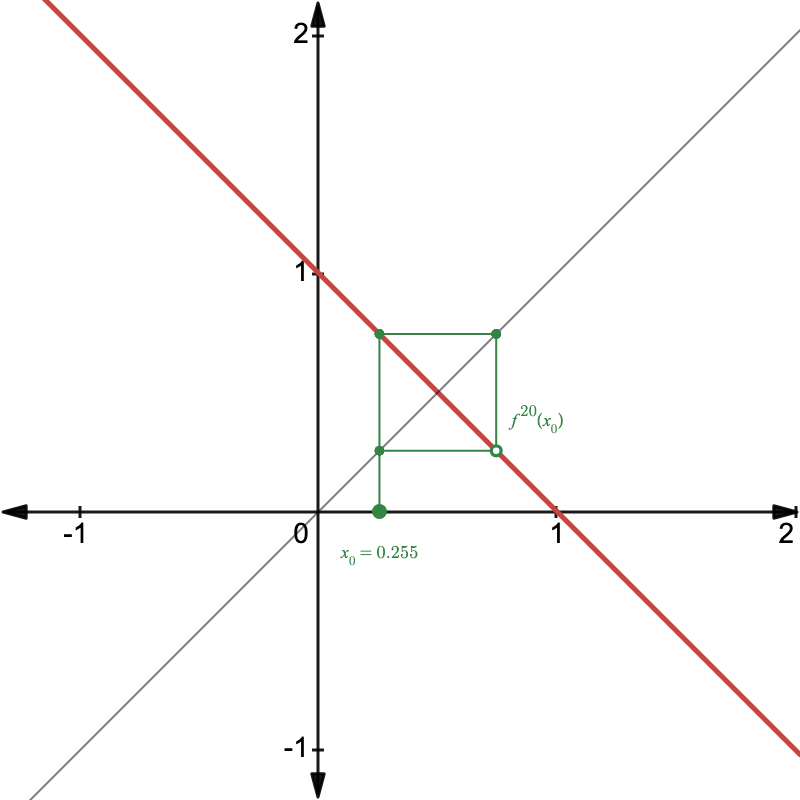
\includegraphics[width=\textwidth]{Grafi/cobweb133.png}
        \caption{\\$g:[0,1] \rightarrow [0, 1]$\\ $x\mapsto 1 - x$}
        \label{fig:cobweb33}
    \end{subfigure}
\end{figure}


$$
h\circ f(x) = g(\sqrt{1 - x^2}) = (\sqrt{1 - x^2})^2 = 1 - x^2 = g(x^2) = g\circ h(x).
$$
Sebi-konjugacija ne ohranja dinamike popolno. V našem primeru je priklopila predperiodične točke, periodičnim.
\end{primer}

\begin{trditev}
Naj bo $g$ semi-konjugirana $f$ preko $h:I \rightarrow J$. Če je $x_0 \in I$ periodična za $f$, je tudi $h(x_0)$ periodična za $g$, a se perioda ne ohranja nujno.
\end{trditev}

\begin{proof}[Dokaz:]
Naj bo $f^n(x_0) = x_0$ in $n\in \N$ najmanjše tako število. Potem velja
\begin{align*}
g^n(h(x_0)) &= g^{n-1}\circ (g\circ h)(x_0) = g^{n-1}\circ (h\circ f)(x_0) = 
\dots = h\circ f^n(x_0) = h(x_0).
\end{align*}
\end{proof}

\begin{opomba}
\hfill
\begin{itemize}
\item Problem je, da nemoremo zagotoviti minimalnosti $n$ za $g$. Recimo, da ima 
$f$ $2$-cikel $\{0, 1\}$, $g$ pa fiksno točko $0$. Če vzamemo $h(0) = h(1) = 0$, bo 
veljalo $h\circ f(0) = 0 = g\circ h(0)$, a ne bosta isti periodi.
\item V splošnem velja, da je perioda delitelj števila $n$.
\end{itemize}
\end{opomba}

\begin{izrek}
Naj bo $g$ semi-konjugirana $f$ s $h: I \rightarrow J$ in naj bosta $I, J \subset \R$ kompaktna intervala in naj bo $f$ kaotičen. Potem je $g$ kaotična, če je izpolnjen eden od treh pogojev:
\begin{enumerate}
\item[i)] $h$ je injektivna
\item[ii)] $g$ je zvezna
\item[iii)] $f$ je zvezna
\end{enumerate}
\end{izrek}

\begin{proof}[Dokaz:]
    ~\\
    \begin{enumerate}
        \item[c1)] Sledi iz trditve. Če vzamemo poljubno $U \subset J$ odprto, je tudi $h^{-1}(U) \subset I$ odprta in vsebuje periodično točko $x_0$. Torej je $h(x_0)$ periodična in v $U$. \\
    \begin{center}
        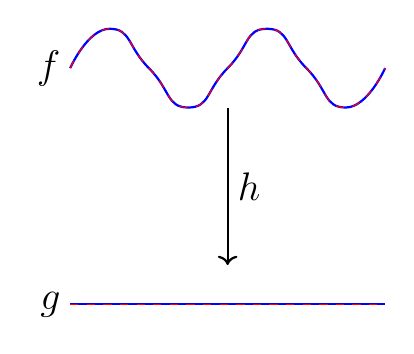
\begin{tikzpicture}
            % Wavy function f
            \draw[thick, blue] plot [smooth, tension=1] coordinates 
            {(0,3) (0.5,3.5) (1,3) (1.5,2.5) (2,3) (2.5,3.5) (3,3) (3.5,2.5) (4,3)};
            
            % Dashed red line following f
            \draw[red, dashed] plot [smooth, tension=1] coordinates 
            {(0,3) (0.5,3.5) (1,3) (1.5,2.5) (2,3) (2.5,3.5) (3,3) (3.5,2.5) (4,3)};
            
            % Label for f
            \node[left] at (0,3) {\Large $f$};
            
            % Straight function g
            \draw[thick, blue] (0,0) -- (4,0);
            \draw[red, dashed] (0,0) -- (4,0);
            
            % Label for g
            \node[left] at (0,0) {\Large $g$};
            
            % Arrow from f to g
            \draw[thick, ->] (2,2.5) -- (2,0.5) node[midway, right] {\Large $h$};
              
        \end{tikzpicture}
     \end{center}
\item[c2)] Če je $O_f(x)$ gosta, je taka tudi $O_g(h(x))$.
\item[c3)] 
\begin{enumerate}
    \item[i)] $h$ je injektivna: 
poglejmo si preslikavo $d: I\times I \rightarrow \R$, podano s predpisom $d(x, y) = |h(x) - h(y)|$. 
Gre za zvezno preslikavo iz kompakta v $\R$. Poglejmo si množico
$$
\Delta_\beta = \{(x, y)\in I\times I \,|\, |x-y| \geq \beta\}.
$$
Ker je $\Delta_\beta$ zaprta in podmnožica $I\times I$ je omejena, torej je kompaktna.
Zato je $I\times I - \Delta_\beta$ kompaktna. Ker je $d$ zvezna, slika $d(I\times I - \Delta_\beta)$
kompaktna. Obstaja $\beta' > 0$: če $|x - y|> \beta$, potem $|h(x) - h(y)| > \beta'$.
Potem iz pogoja $|f^n(x) - f^n(y)| > \beta$ sledi $|g^n(h(x)) - g^n(h(y))| > \beta'$. To je občutljivostna konstanta za $g$.
\item[ii)] $g$ je zvezna: ker je $g$ zvezna pogoj $c3)$ sledi iz $(c1)$ in $(c2)$.
\item[iii)] $f$ je zvezna (ideja): zaradi konjugacije obstaja osprta $U \subset J$, ki ima 
do $m$ praslik. Zaradi kompaktnosti, zveznosti $h$ in lokalne obrljivosti, obstaja 
$\delta > 0$, da iz diam$(U) < \delta$ sledi, da imajo praslike diam$(g^n(U)) < \delta$
za vse $n\in \N_0$. Zaradi zveznosti se praslike $g^n(U)$ slikajo v $g^{nm}(U)$. 
Torej obstaja praslika $V$ od $U$, da je diam$(f^n(V))< \beta$ za vse $n\in \N_0$, 
kar je protislovje. 
\end{enumerate}
\end{enumerate}
\end{proof}

\begin{opomba}
Zakaj je pomembna kompaktnost intervalov $I$ in $J$? Poglejmo si preslikavi 
\begin{align*}
&f(x) = 2x \text{ na } (0, \infty) \\ 
&g(x) = x + \ln 2 \text{ na } \R.
\end{align*}
Očitno je, da je $f$ izpolnjuje $(c3)$, saj sta za velik $n$ števili $2^n x$ in $2^n y$ daleč narazen, če $x\neq y$. Po drugi strani, je tudi očitno, da $g$ ne izpolnjuje $(c3)$, saj je razlika 
$$
|g^n(x) - g^n(y)| = |x + n\ln(2) - (y + n\ln(2))| = |x-y|
$$
konstantna za vse $n\in \N$. Sta pa vseno $f$ in $g$ konjugirani preko $h(x) = \ln(x)$.
$$
g(x) = h\circ f\circ h^{-1}(x) = \ln(2e^x) = \ln(e^x) + \ln(2) = x + \ln(2).
$$.
\end{opomba}

\begin{primer}
Poglejmo si sedaj primere semi-konjugacije na Podvojitveni in šotorasti preslikavi. 
\begin{align*}
&D(x) = 2x - \lfloor 2x \rfloor \\ 
&T(x) = 2\min\{x, 1-x\}
\end{align*}
Imamo 
$$T(D(x)) = 2\min\{D(x), 1 - D(x)\} = T(T(x))$$.
To pomeni, da je $T$ semi-konjugirana $D$ za $h = T$. Posledično kaotičnost 
$T$ sledi.
\end{primer}

\begin{primer}
Imamo preslikavo
\begin{align*}
&h: [0, 1) \rightarrow S^1 \subset \R^2 \\ 
&h(x) = (\cos{2\pi x}, \sin{2\pi x})
\end{align*}
Zanima nas, kaj se zgodi z doubling map, če uporabimo to konjugacijo oz. trdimo, da bo konjugirana preslikava 
\begin{center}
    \begin{tikzpicture}
    
        % Interval representation
        \draw[thick] (0,2) -- (4,2);
        \filldraw (0,2) circle (1.5pt) node[below] {0};
        \filldraw (4,2) circle (1.5pt) node[below] {1};
        \filldraw (2,2) circle (1.5pt) node[below] {$\frac{1}{2}$};
    
        \draw[->,red,thick] (0,2) -- (2,2);
        \draw[->,orange,thick] (2,2) -- (4,2);
    
        % Mapping downwards
        \draw[->] (2,0.5) -- (2,-1) node[midway,right] {$D$};
    
        % Mapped interval
        %\draw[thick] (0,0) -- (4,0);
        %\filldraw (0,0) circle (1.5pt);
        %\filldraw (4,0) circle (1.5pt);
    
        \draw[->,red,thick] (0,-2) -- (2,-2);
        \draw[->,orange,thick] (2,-2) -- (4,-2);
    
        % Arrow indicating a function
        \draw[->] (5.5,1.8) -- (7.5,1.8) node[midway,above] {$h$};
        \draw[->] (5.5,-2) -- (7.5,-2) node[midway,above] {$h$};
    

        % Circles
        \draw[thick] (10,2) circle (1pt);
        \draw[->,red,thick] (10+1,2) arc (0:180:1);
        \draw[->,orange,thick] (10-1,2) arc (180:360:1);
    
        \draw[->] (10,0.5) -- (10,-0.5) node[midway,right] {$f$};
    
        \draw[thick] (10,-2) circle (1pt);
        \draw[->,red,thick] (10+1,-2) arc (0:180:1);
        \draw[->,orange,thick] (10-1,-2) arc (180:360:1);
    
    \end{tikzpicture}
\end{center}

Sklep: $D$ je konjugirana $f: S^1 \rightarrow S^1$, $f(\cos{t}, \sin{t}) = (\cos{2t}, \sin{2t})$
za $t\in [0, 2\pi]$ tj. preslikavi ki podvoji argument. V kompleksni notacijo bi j
o zapisali z $e^{it} \mapsto e^{2it}$ ali $z \mapsto z^2$. Posledično je tudi $f$
kaotična.
\end{primer}

\begin{primer}
Pokažimo, da je $q_{-2}(x) = x^2 - 2$ kaotična. To bo sledilo iz dejstva, da je 
semi-konjugirana preslikavi podvojitev argumenta, preko semi-konjugacije $h$ 
\begin{align*}
h: S^1 \rightarrow [-2, 2] \\ 
(x, y) \mapsto 2x 
\end{align*}
Ta preslikava ima v vsaki točki $y\in [-2, 2]$ največ $2$ prasliki, je zvezna in 
surjektivna. Preverimo, da komutirata $g$ in $q_{-2}$:
\begin{align*}
h\circ g(\cos{2t}, \sin{2t}) &= 2\cos{2t} = 2\cos^2{t} - 2\sin^2{t} = 4\cos^2{t} - 2\\
q_{-2}\circ h(\cos{t}, \sin{t}) &= q_{-2}(2\cos{t}) = 4\cos^2{t} - 2 = 4\cos^2{t} - 2
\end{align*}
Sklep: $q_{-2}$ je semi-konjugirana $D$. Direktna preslikava bi bila 
$$
h(x) = 2\cos(2\pi x).
$$
Ker je $q_{-2}$ zvezna, po prejšnjem izreku je tudi kaotična.
\end{primer}

\section{Bifurkacije}

Za motivacijo si oglejmo enoparametrično družino šotorskih preslikav za $c\in [0, 2]$:
$$
T_c(x) = \frac{c}{2}\cdot \min\{x, 1-x\} = \frac{c}{2} T(x).
$$
Vse te preslikave interval $[0, 1]$ slikajo vase, dinamike pa se za različne vrednosti malce razlikujejo
\newpage
\begin{itemize}
\item če je $c < 1$: 
\begin{figure}[h!]
    \begin{center}
        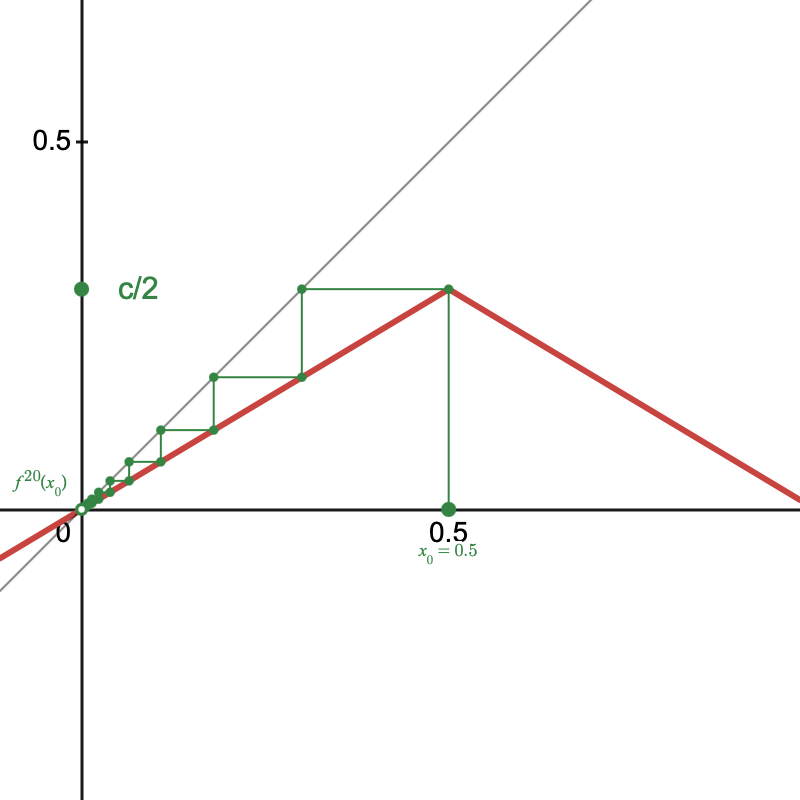
\includegraphics[width=6cm, height=5.5cm]{Grafi/cobweb141.png}
        %\caption{pajčevinast diagram iz Primera 3.}
    \end{center}
\end{figure} 

$x_0$ je edina periodična točka, gre pa za privlačno fiksno točko, saj je $T_c'(0) = c < 1$.
\item če je $c = 1$: 
\begin{figure}[h!]
    \begin{center}
        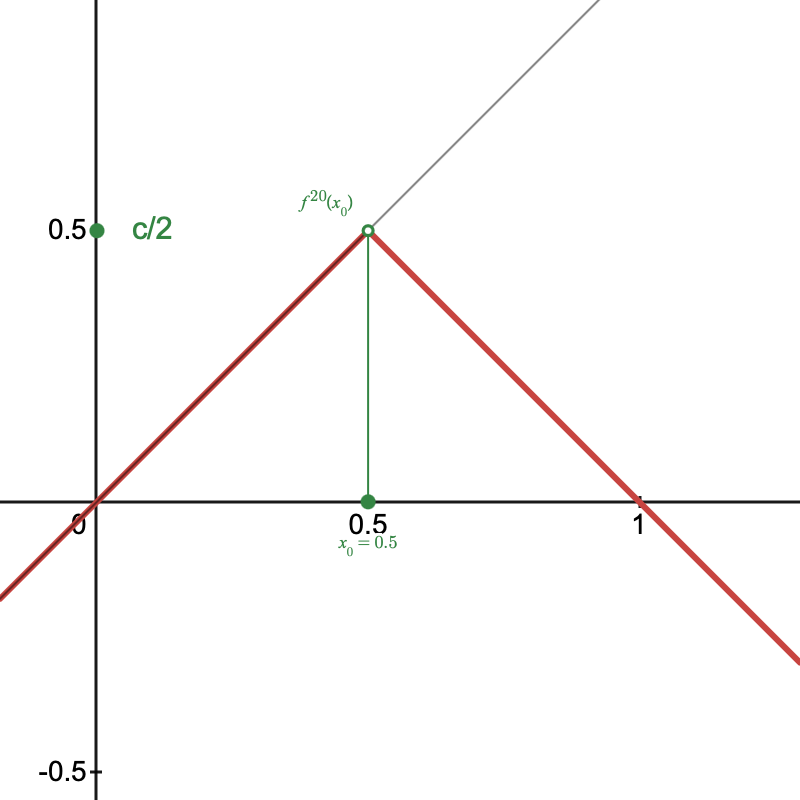
\includegraphics[width=6cm, height=5.5cm]{Grafi/cobweb142.png}
        %\caption{pajčevinast diagram iz Primera 3.}
    \end{center}
\end{figure}
\newpage
\item če je $c\in (1, 2]$: 
\begin{figure}[h!]
    \begin{center}
        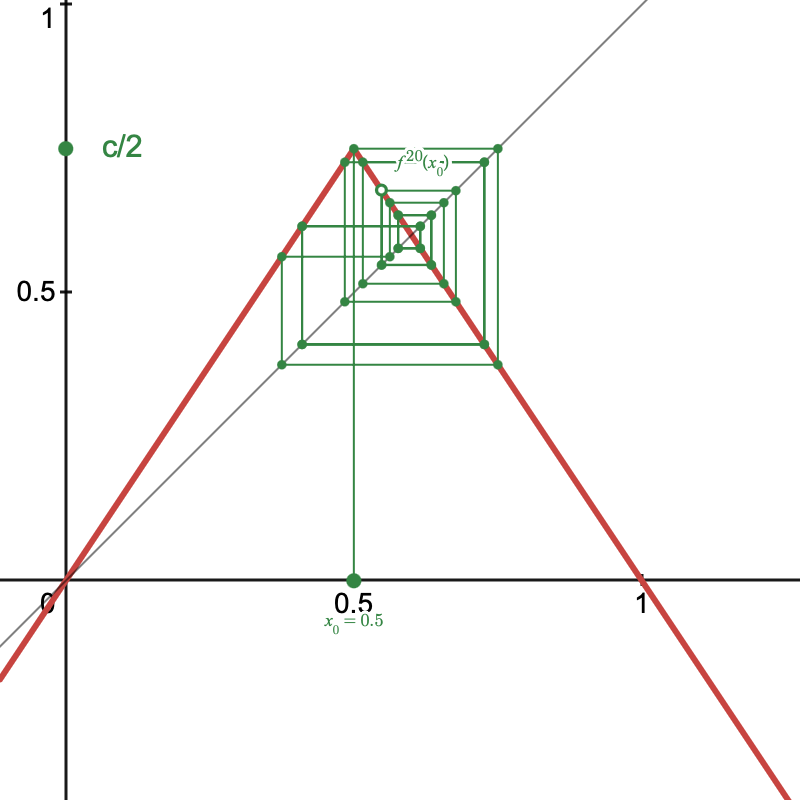
\includegraphics[width=6cm, height=5.5cm]{Grafi/cobweb143.png}
        %\caption{pajčevinast diagram iz Primera 3.}
    \end{center}
\end{figure}

pojavi se dodatna fiksna točka 
$$
c - cx = x \iff x = \frac{c}{1 + c}.
$$
Ta točka je odbojna , saj je na $(\frac{1}{2}, 1]$ odvod $T_c'(x) = -c < -1$. 
Opazimo, da je $x = 0$ postala odbojna točka, saj $T_c'(0) = c > 1$.
\end{itemize}
\noindent
Opazka: ob prehodu čez $c=1$ je prišlo do kvalitativne spremembe dinamike, saj 
smo iz ene dobili dve fiksni točki.

\noindent
Poglejmo si kaj se dogaja z $2$-cikli oz. $T_c^2$:
$$
T_c^2(x) = c\cdot \min\{ T_c(x), 1 - T_c(x)\}
$$
Za $c < 1$ nimamo presečišč z $y = x$ zato se omejimo na $c \geq 1$. Za $c=1$
so vsa presečišča fiksne točke. Ob prehodu čez $c = 1$ pa iz točke $x = \frac{1}{2}$
dobimo dve $2$-periodični točki.
\begin{figure}[h!]
    \begin{center}
        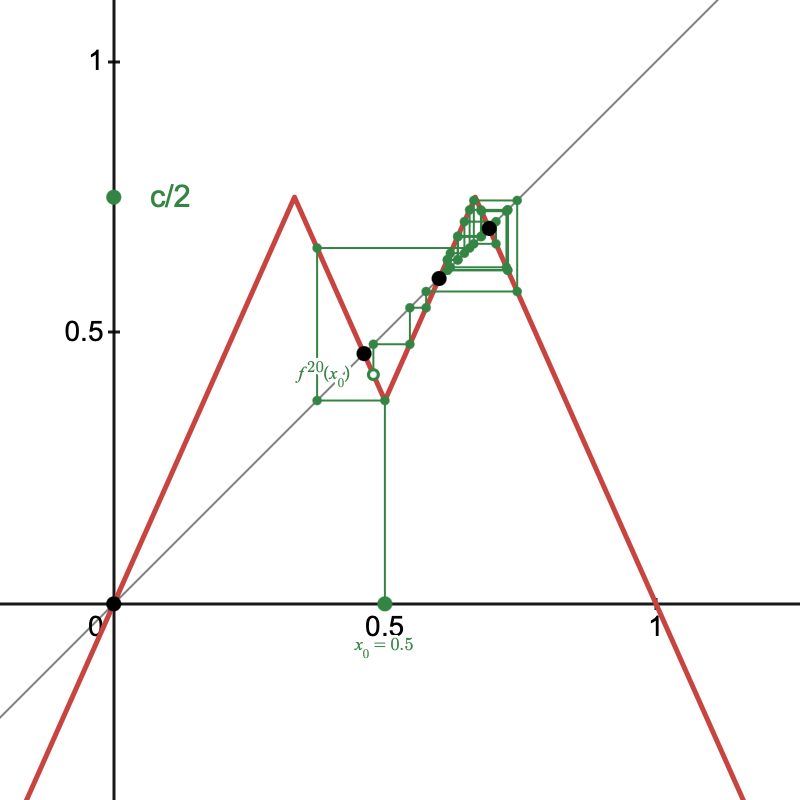
\includegraphics[width=6cm, height=4.6cm]{Grafi/cobweb15.png}
        %\caption{pajčevinast diagram iz Primera 3.}
    \end{center}
\end{figure}
\noindent
\newpage
Za $T_c^3$ postane obnašanje še bolj zanimivo 
\begin{figure}[h!]
    \begin{center}
        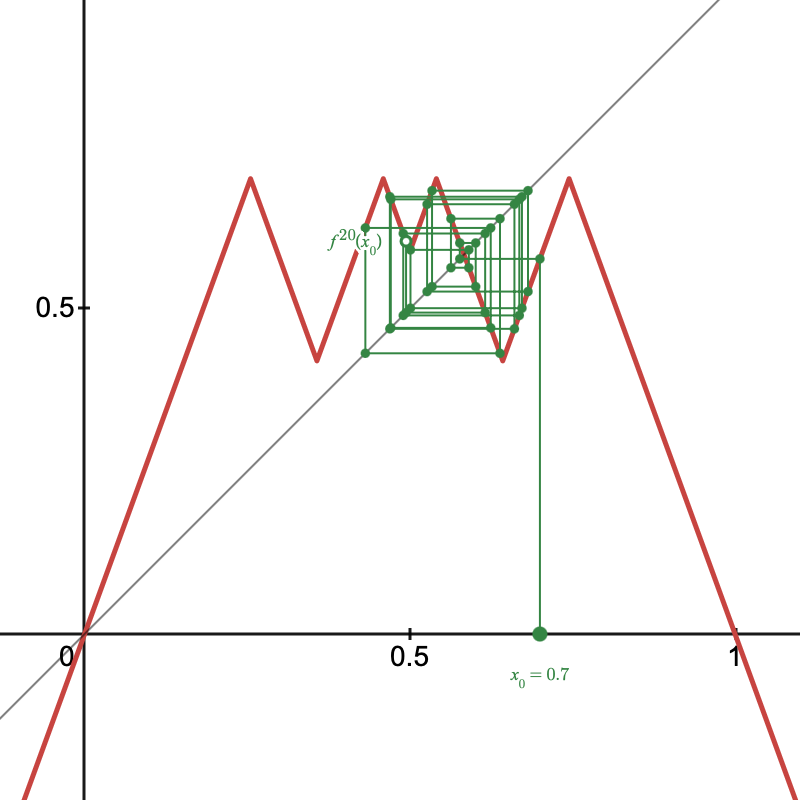
\includegraphics[width=6cm, height=5.5cm]{Grafi/cobweb16.png}
        %\caption{pajčevinast diagram iz Primera 3.}
    \end{center}
\end{figure}
Izkaže se, da pri $c = \frac{1 + \sqrt{5}}{2}$ sekamo $T^3$ natanko $5$-krat 
($3$-cikel $+$ $2$ fiksni točki). Pri večjih je presečišč $8$ (dva $3$-cikla) 
pri manjših pa $2$. Kasneje bomo dokazali, da se ob $3$-ciklu pojavijo še vse 
ostale periode.
Točkam, pri katerih se zgodi "kvalitativna sprememba" dinamike, pravimo bifurkacije.
\newline
Formalno:

Obravnavamo družino zveznih funkcij $f_c: I \rightarrow I \subset \R$, 
za parametr $c\in J \subset \R$. Ta družina je $C^k$-odvisna od $c$, če 
$k$-ti parcialni odvodi $F(x, c) \coloneqq f_c(x)$ obstajajo
$\frac{\partial^k}{\partial c^k} F(x, c)$ in so zvezni, za $k\in \N_0$. 
Na primer $T_c(x) = \frac{c}{2} T(x)$ je taka, čeprav ni odvedljiva po $x$ v 
$x = \frac{1}{2}$ in velja
\begin{align*}
&\frac{\partial}{\partial c} T_c(x) = \frac{1}{2} T(x) \\ 
&\frac{\partial^k}{\partial c^k} T_c(x) = 0, \,\, k \geq 2.
\end{align*}

\begin{definicija}
Vrednosti $c\in J$ pravimo \textbf{bifurkacija} družine $f_c$, če se dinamika 
ob prehodu čez njo kvalitativno spremeni.
\end{definicija}

Pri motivaciji smo opazili različne tipe bifurkacij:
\begin{itemize}
\item Fiksna točka se je pojavila in izginila (npr. $x = \frac{1}{4}$ pri $c=1$).
\item Fiksna točka se je pojavila in nato podvojila (za $c = \frac{1 + \sqrt{5}}{2}$ in poljubni fiksni točki)
\item Iz fiksne točke $x = \frac{1}{2}$, ki se pojavi pri $c = 1$, smo dobili fiksno točko drugega tipa in $2$-cikel.
\end{itemize}
Ključna opazka je, da so se spremembe zgodile, ko je odvod v fiksni točki $1$ ali pa ne obstaja.

\begin{izrek}
Naj bo $f_c: I \rightarrow I$ družina zvezno odvedljivih funkcij, ki so gladko odvisne od parametra $c\in J$. Denimo, da za $x_0 \in I$ velja $f_{c_0}(x_0) = x_0$ in $f_{c_0}'(x_0) \neq 1$. Potem obstajata okolica $I' \subset I$ in $J' \subset J$, ter preslikava $p: J' \rightarrow I'$, da je $f_c(p(c)) = p(c)$, za katero je $p(c)$ edina fiksna točka na $I'$ pri $c\in J'$. 
\end{izrek}

\begin{proof}[Dokaz:]
Uporabimo izrek o implicitni preslikavi za 
$$
F(x, c) = f_c(x) - x.
$$
Po predpostavki je:
\begin{align*}
F(x_0, c_0) = 0 \text{ in } \frac{\partial}{\partial x} F(x_0, c_0) = f_{c_0}'(x_0) - 1 \neq 0. 
\end{align*}
Torej lahko na majhni okolici $c_0 \in J$ izrazimo $x = p(c)$, ter velja $F(p(c), c) = 0$ oz. $f_c(p(c)) = p(c)$.
\end{proof}

\begin{opomba}
Izrek podaja le potreben, ne pa tudi zadosten pogoj.
\end{opomba}

\begin{posledica}
Privlačne in odbojne fiksne točke se pri majhnih motnjah ohranijo. Enako velja 
za točke, kjer je odvod $-1$. Pri nevtralnih točkah z odvodom $+1$ pa lahko pride 
do sprememb.
\end{posledica}

\begin{primer}[Tangentna bifurkacija]
Bifurkacija, v katerih iz nevtralne točke, ki zadošča $f_{c_0}'(x_0) = 1$, 
dobimo dve fiksni točki, ki jih prej ni bilo. Ena je privlačna, druga odbojna, 
zato se tudi imenuje saddle-node bifurcation. 
Opazujemo družino $g_c(x) = x^2 + c$. Dobimo 
\begin{itemize}
    \item za $c > \frac{1}{4}$ ni fiksnih točk 
    \item za $c = \frac{1}{4}$ se pojavi nevtralna točka 
    \item za $c < \frac{1}{4}$ se razcepi v privlačno in odbojno točko.
\end{itemize}
\end{primer}

\begin{primer}[Potrojitev fiksnih točk]
Imamo družino $f_c(x) = c\arctan{x}$ za $c\in [0, \infty]$.
\end{primer}

\begin{figure}[h]
    \centering
    % First figure
    \begin{subfigure}[c]{0.28\textwidth}
        \centering
        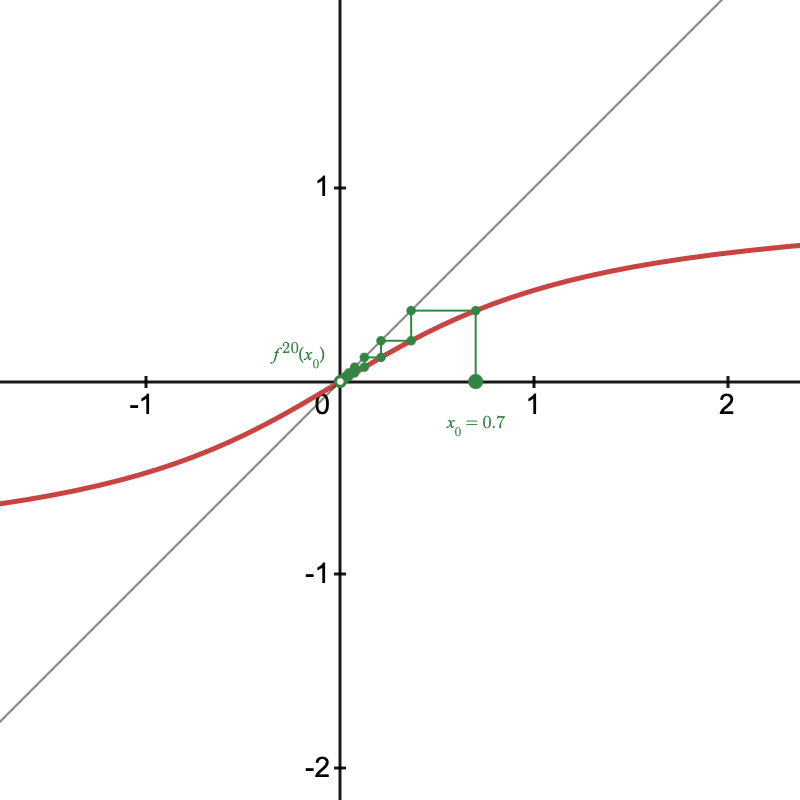
\includegraphics[width=\textwidth]{Grafi/cobweb171.png}
        \caption{\\$c<1$ privlačna}
        \label{fig:cobweb31}
    \end{subfigure}
    % Second figure
    \begin{subfigure}[c]{0.28\textwidth}
        \centering
        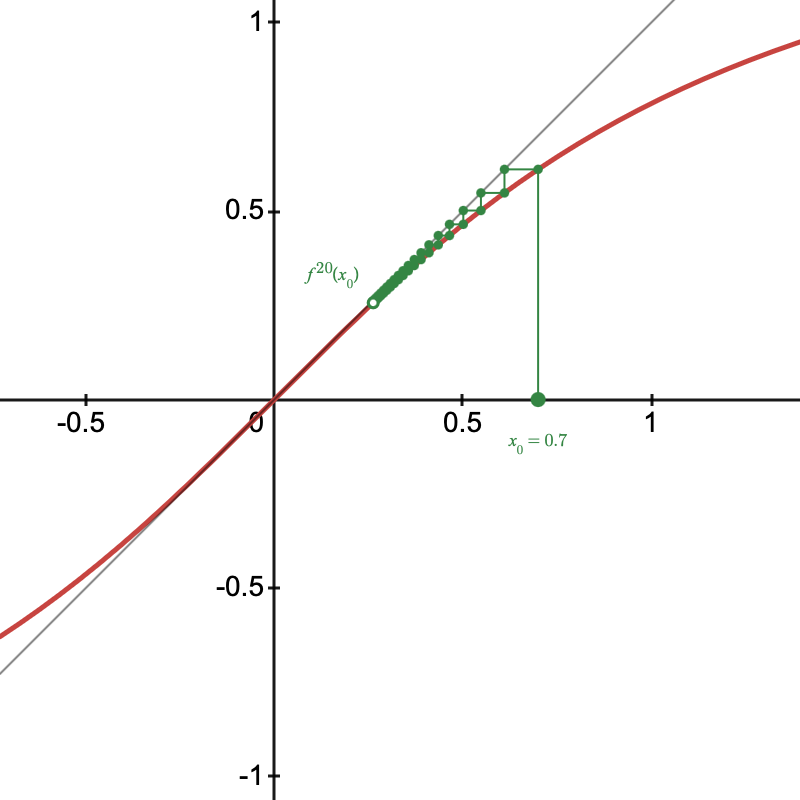
\includegraphics[width=\textwidth]{Grafi/cobweb172.png}
        \caption{\\$c=1$ nevtralna in\\šibko privlačna}
        \label{fig:cobweb32}
    \end{subfigure}
    % Third figure
    \begin{subfigure}[c]{0.28\textwidth}
        \centering
        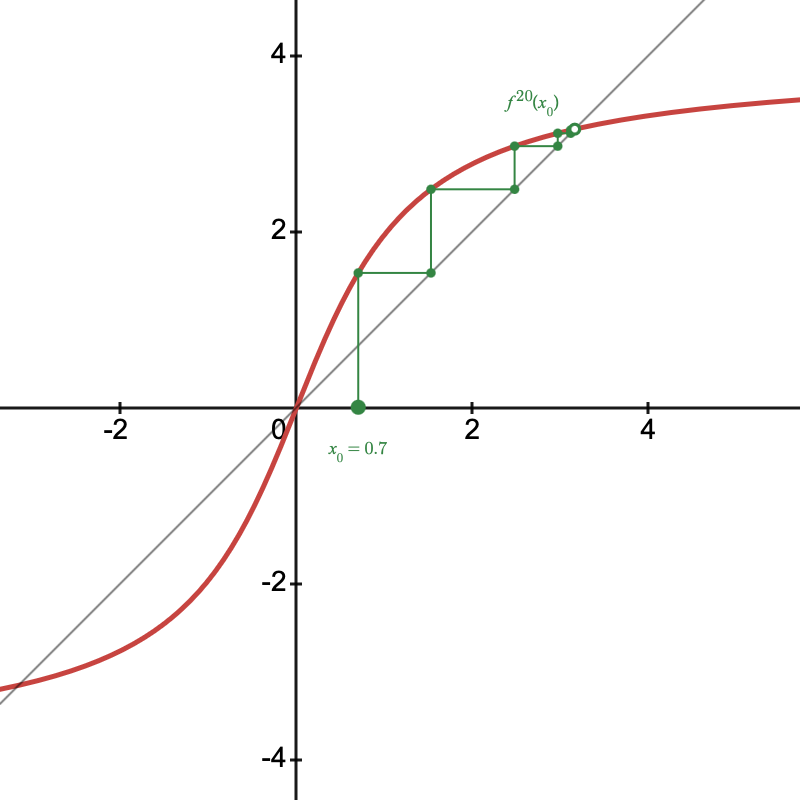
\includegraphics[width=\textwidth]{Grafi/cobweb173.png}
        \caption{\\$c>1$ odbojna in\\dve privlačni}
        \label{fig:cobweb33}
    \end{subfigure}
\end{figure}



% Uncomment the following two lines if you want to have a bibliography. Please do not forget to add an entry to your bibliography and reference it by using the \cite{} command
%\bibliographystyle{alphadin}
%\bibliography{document}

% End of the document
\end{document}
